%% Secure-first Methodology for IoT Ecosystems
%% Target journal: Computers & Security (Elsevier), Q1, IF ~5.6
%% Template: elsarticle (Elsevier standard)
%%
%% COMPILATION NOTES
%%   1. Copy sn-bibliography.bib from ../Context/metodologia v2 Springer/v3/ and rename to references.bib
%%      OR update \bibliography{} command below with the relative path.
%%   2. Figures referenced with relative paths:
%%         ../Context/metodologia v2 Springer/v3/Methodology v2.pdf
%%         ../Context/metodologia v2 Springer/v3/Methodology identity parameters.pdf
%%   3. Placeholder values marked \ph{...} must be replaced with real hardware measurements
%%      before submission.
%%   4. TODO comments mark sections requiring content additions before submission.
%%
%% STATUS: Draft — timing/heap/chain data updated from 2026-07-15 multi-run experiments (2 NODE_02 runs, 196 pooled bench msgs + 1 NODE_01 recovery run, 120 bench msgs).
%%          Expert questionnaire results incorporated (N=14, mean 3.98/5) as of 2026-09-15 (panel expanded 2026-08-19 – 2026-09-15; majority independent: 8/14).
%%          Companion code repository published 2026-08-18 (Apache-2.0); paper-artifact repository published 2026-09-21.
%%          2026-09-28: Root of Trust redesigned from PSK+NVS to a PUF-based scheme (esp32_puflib, Stanicek/CTU FIT 2022; SRAM PUF on ESP32 RTC FAST memory).
%%          2026-09-28 (correction pass): firmware is C/ESP-IDF (NOT MicroPython) throughout; blake3 is not used; the SecureNode-derived hash-chain
%%          audit mechanism (M_num, PRV_bl, P4 Data Exchange/P5 Logout/P6 Chain Audit) has been dropped in favor of a 3-phase design
%%          (P1 Enrollment, P2 Root of Trust via nonce-based hash-reconstruction challenge, P3 AES-256-GCM data exchange). This trades away the
%%          cryptographic chain-of-custody previously claimed for Repudiation/I8; see the Limitations bullet documenting this trade-off.
%%          All narrative/protocol/table sections not requiring new bench data were updated; sections still describing the prior PSK+NVS empirical results
%%          (Abstract numbers, Tables csq3a/csq3b, tab:functional Pass results, expert-survey items B7/B9/B10) are marked with
%%          "%% PENDING-PUF-DATA" comments and/or \ph{} placeholders pending firmware implementation and new bench trials.
%%          2026-10-02: first N=30 real-hardware PUF bench (SMG_NODE_01 vs. real RPi4 server) completed; Table tab:pufbench added.
%%          2026-10-05/06: second critical-review pass on the PUF redesign (ERRATA.md Section F) — all findings resolved except one
%%          (artifact-repository publication for the PUF redesign, ERRATA.md F.4, pending explicit author confirmation before a public
%%          GitHub push). As part of this pass: a firmware debug print of the raw session verifier was removed (production hygiene) and a
%%          boot-log label fixed; because this changed the archived firmware after the first bench round, that round was discarded and a
%%          fresh, independent N=30 hard-reset bench was run (2026-10-06) against the current firmware — Table tab:pufbench, the Abstract,
%%          Conclusion, and all cross-referencing rows now report this second round's figures exclusively. SMG_NODE_02 remains untested
%%          under the PUF scheme; a formal min-entropy assessment (NIST SP 800-90B) and thermal/voltage sensitivity testing remain open
%%          (see the 2 remaining \ph{} markers). main.tex recompiles clean: 64 pages, 0 undefined references/citations
%%          (pdflatex->bibtex->pdflatex x2, verified 2026-10-06).

\documentclass[preprint,12pt,authoryear]{elsarticle}

\usepackage{graphicx}
\usepackage{multirow}
\usepackage{amsmath,amssymb,amsfonts}
\usepackage{amsthm}
\usepackage[title]{appendix}
\usepackage{xcolor}
\usepackage{booktabs}
\usepackage{enumitem}
\usepackage{threeparttable}
\usepackage{caption}
\usepackage{pifont}
\usepackage[utf8]{inputenc}
\usepackage[T1]{fontenc}
\usepackage{array}
\usepackage{rotating}
\usepackage{tabularx}
\usepackage{siunitx}
\usepackage{makecell}
\usepackage{longtable}
\usepackage{tikz}
\usetikzlibrary{shapes.geometric, arrows.meta, positioning, calc, backgrounds, decorations.pathreplacing, fit}
\usepackage[colorlinks=true,linkcolor=blue,citecolor=blue,urlcolor=blue]{hyperref}
\usepackage{soul}    % for \hl{}

%% Check/cross marks for comparison tables
\newcommand{\cmark}{\ding{51}}
\newcommand{\xmark}{\ding{55}}
\definecolor{checkgreen}{RGB}{0,128,0}
\definecolor{crossred}{RGB}{180,0,0}
\definecolor{partialyellow}{RGB}{180,120,0}
\newcommand{\yes}{\textcolor{checkgreen}{\cmark}}
\newcommand{\no}{\textcolor{crossred}{\xmark}}
\newcommand{\pyes}{\textcolor{partialyellow}{\textasciitilde}}

%% Hardware-pending placeholder macro.
%% Usage: \ph{describe what measurement replaces this}
%% Remove before submission.
\definecolor{phbg}{RGB}{255,230,100}
\newcommand{\ph}[1]{\colorbox{phbg}{\small\texttt{[TODO: #1]}}}

\renewcommand{\topfraction}{0.85}
\renewcommand{\textfraction}{0.1}
\setcounter{topnumber}{4}
\setcounter{totalnumber}{6}

\newtheorem{definitions}{Definition}

\journal{Computers \& Security}

\begin{document}

\begin{frontmatter}

\title{Closing the Security Activation Gap: A Security-by-Design Methodology for IoT Ecosystems and Its Empirical Validation in a DC Smart Microgrid}

\author[inaoe1,inaoe2]{Raziel Campos-Sanchez\corref{cor1}}
\ead{rcampos@inaoe.mx}
\cortext[cor1]{Corresponding author}

\author[inaoe1]{Luis Hernandez-Martinez}
\ead{luish@inaoe.mx}

\author[inaoe2,inaoe3]{Claudia Feregrino-Uribe}
\ead{cferegrino@inaoe.mx}

\author[ceit,unad]{Alejandro Penuelas-Angulo}
\ead{apenuelasan@ceit.es}

\author[inaoe2,inaoe3]{Diego Cruz-Aguilar}
\ead{diego.cruz@inaoe.mx}

\affiliation[inaoe1]{organization={Electronics Department, National Institute of Astrophysics, Optics and Electronics (INAOE)},
    addressline={Luis Enrique Erro 1},
    city={San Andr\'{e}s Cholula},
    postcode={72840},
    state={Puebla},
    country={Mexico}}

\affiliation[inaoe2]{organization={Science and Technologies of Security Department, INAOE},
    addressline={Luis Enrique Erro 1},
    city={San Andr\'{e}s Cholula},
    postcode={72840},
    state={Puebla},
    country={Mexico}}

\affiliation[inaoe3]{organization={Computational Sciences Department, INAOE},
    addressline={Luis Enrique Erro 1},
    city={San Andr\'{e}s Cholula},
    postcode={72840},
    state={Puebla},
    country={Mexico}}

\affiliation[ceit]{organization={CEIT-Basque Research and Technology Alliance (BRTA)},
    addressline={Manuel Lardizabal 15},
    city={Donostia/San Sebasti\'{a}n},
    postcode={20018},
    state={Guipuzcoa},
    country={Spain}}

\affiliation[unad]{organization={Universidad de Navarra, Tecnum},
    addressline={Manuel Lardizabal 15},
    city={Donostia/San Sebasti\'{a}n},
    postcode={20018},
    state={Guipuzcoa},
    country={Spain}}

\begin{abstract}
A persistent security activation gap constrains the widespread adoption of IoT ecosystems: security mechanisms are widely available in commercial platforms yet remain inactive after standard deployment. Closing this gap requires not only improved tools but also a methodology that embeds cybersecurity as a foundational design concern from the earliest development stages. We present a security-by-design methodology for centralized IoT ecosystems that treats identity as an intrinsic entity property, spans seven stages across four phases, and integrates cybersecurity throughout the development lifecycle. A dynamic Root of Trust process establishes verifiable cryptographic identity for each entity, providing the trusted foundation for authentication, access control, and secure communication.

We validate the methodology through a confirmatory case study \citep{yin2014case} applying all seven stages to the design and implementation of a DC Smart Microgrid (SMG): an industrial IoT ecosystem comprising two ESP32-based secondary control nodes and a Raspberry Pi~4B primary coordination agent. Four case study questions (CSQ1--CSQ4) evaluate guidance sufficiency, identity model unambiguity, Root of Trust verifiability, and threat coverage. Results show that all seven stages produced documented, traceable artifacts with no external guidance required (CSQ1); that a 14-parameter identity model across four entity types was produced without ambiguity (CSQ2); that the Root of Trust process established mutual authentication with a 56.7\,ms total P2+P3 handshake latency (averaged across two independent bench runs), a per-message P4 latency of $30.3 \pm 3.3$\,ms (196 pooled bench messages, NODE\_02), and 100\% chain integrity with zero security errors (CSQ3); %% REDLINE M3+M4+E3
and that the methodology achieves unweighted OWASP IoT Top~10 coverage of 7/10 items fully addressed and 3/10 partially addressed---I4 secure-update policy only, I8 device management without a cryptographically verifiable chain, and I10 physical hardening outside software scope (CSQ4). The CSQ3 figures above describe the case study's original PSK+NVS Root of Trust instantiation; a subsequent PUF-based redesign (Section~\ref{sec:methodology}) was independently validated end-to-end on real hardware for one of the two SMG nodes ($N=30$ hard-reset trials against a real WiFi access point and a real primary-agent server): 30/30 end-to-end success, mean mutual-authentication handshake latency $80.7 \pm 36.2$\,ms, with PUF-response reconstruction requiring exactly two attempts in every trial (Section~\ref{subsec:pufbench}); validation of the second node, and full replacement of the CSQ3 figures above, remain future work. The methodology's parameterized, technology-agnostic structure is designed to generalize across diverse IoT application domains; empirical validation in additional domains remains future work.
\end{abstract}

\begin{keyword}
Internet of Things \sep Security-by-Design \sep IoT Methodology \sep Root of Trust \sep Identity Management \sep Smart Microgrid \sep Case Study Research
\end{keyword}

\end{frontmatter}


% ============================================================
\section{Introduction}
\label{sec:introduction}
% ============================================================

The Internet of Things (IoT) has evolved from a conceptual vision into a technological paradigm underpinning critical infrastructure, industrial automation, healthcare systems, and smart cities \citep{al2015internet, zhou2021internet}. Despite this expansion, large-scale IoT adoption remains constrained by fragmented architectures, heterogeneous technologies, and---critically---the failure to integrate cybersecurity from the earliest design stages \citep{shahinzadeh2024security, makhdoom2018anatomy}.

The consequences of this gap are well documented. The Mirai botnet, which compromised over 600,000 IoT devices to launch unprecedented distributed denial-of-service attacks, originated from misconfigured or unprotected deployments relying on default credentials \citep{Mirai_analysis_2017}. Subsequent analyses confirm that cyberattacks on IoT infrastructure continue to escalate in frequency and sophistication, targeting energy systems, healthcare networks, and public utilities \citep{abraham2025cyber, okika2025addressing}.

A central observation motivating this work is that the principal barrier to secure IoT deployment is not the \emph{absence} of security features but the \emph{security activation gap}: the disconnect between security capabilities \emph{available} in a platform and those \emph{operational} after a standard deployment (Figure~\ref{fig:gap}). Widely adopted open-source IoT platforms provide security mechanisms that require manual post-installation configuration, effectively restricting their use to organizations with dedicated security expertise \citep{NIST_IoT_2020}.

A second, more fundamental barrier operates at the methodological level: most IoT development projects lack a structured process that integrates cybersecurity from organizational decision-making through operational maintenance. Security is typically addressed \emph{after} architectural and technology decisions are made, producing mechanisms that are bolt-on rather than foundational, with identity management that is platform-specific rather than entity-centric.

To address both barriers, we present two complementary contributions:

\begin{enumerate}
    \item \textbf{A security-by-design methodology} for developing centralized IoT ecosystems. The methodology treats identity as an intrinsic property of every entity, spans seven stages across four phases (organizational strategy, architecture, implementation, and operation), and embeds cybersecurity---from threat policy to Root of Trust establishment---as a foundational concern from problem definition through ongoing operation. A dynamic Root of Trust (RoT) process establishes verifiable cryptographic identity for each entity before any operational communication begins.

    \item \textbf{An empirical confirmatory case study} applying the methodology to the design and implementation of a DC Smart Microgrid (SMG) IoT ecosystem, following Yin's \citeyearpar{yin2014case} Case Study Research design. The SMG comprises two ESP32 secondary control nodes and a Raspberry Pi~4B primary coordination agent, reaching Technology Readiness Level~3. Four case study questions evaluate guidance sufficiency, identity model unambiguity, Root of Trust verifiability, and OWASP IoT threat coverage.
\end{enumerate}

\noindent\textbf{Conceptual foundation:} The identity-centric IoT paradigm, the IoT/ecosystem distinction, the formal entity identity model, and the reconceptualization of the Root of Trust as a multi-phase process are established at the conceptual and definitional level in a companion manuscript \citep{campos2026identity}. The present work builds directly on that foundation to specify, validate, and empirically evaluate an operative seven-stage development methodology; it does not re-derive these definitions independently.

\begin{figure}[htbp]
    \centering
    % Figure: The Security Activation Gap
% Side-by-side comparison: standard IoT deployment vs. methodology-driven.
% Left column: some security controls available but not activated.
% Right column: all controls activated by design through the methodology.
% The gap is shown as a bi-directional annotation between the two.

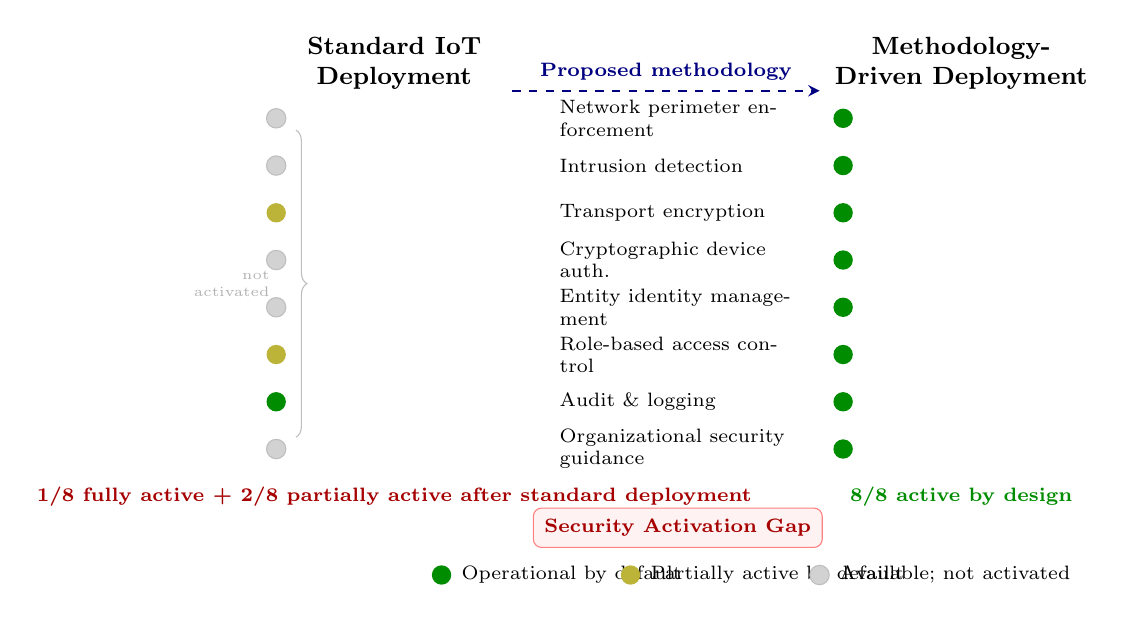
\begin{tikzpicture}[font=\footnotesize]

% ── Styles ──────────────────────────────────────────────────
\tikzset{
  colbox/.style={draw=gray!50, fill=gray!4, rounded corners=5pt,
                 minimum width=3.8cm, inner sep=8pt},
  hdr/.style={font=\bfseries\small, align=center, text width=3.6cm},
  rowlabel/.style={align=left, text width=3.0cm, font=\scriptsize},
  doton/.style={circle, fill=green!55!black, minimum size=7pt, inner sep=0pt},
  dotoff/.style={circle, fill=gray!35, draw=gray!50, minimum size=7pt, inner sep=0pt},
  dotpartial/.style={circle, fill=yellow!70!black, minimum size=7pt, inner sep=0pt},
  gaparrow/.style={<->, very thick, >=stealth, red!65!black},
  methodarrow/.style={->, thick, >=stealth, blue!50!black, dashed}
}

% ── Column x-positions ──────────────────────────────────────
\def\lx{0}      % left column centre
\def\rx{7.2}    % right column centre
\def\dotlx{-1.5}% left dot x
\def\dotrx{5.7} % right dot x
\def\lbllx{-1.1}% left label x
\def\lblrx{6.1} % right label x

% ── Row y-positions (8 controls) ────────────────────────────
\def\rowA{-0.7}
\def\rowB{-1.3}
\def\rowC{-1.9}
\def\rowD{-2.5}
\def\rowE{-3.1}
\def\rowF{-3.7}
\def\rowG{-4.3}
\def\rowH{-4.9}

% ── Column headers ───────────────────────────────────────────
\node[hdr] at (\lx, 0)  {Standard IoT Deployment};
\node[hdr] at (\rx, 0)  {Methodology-Driven Deployment};

% ── Control labels (shared between columns) ──────────────────
\node[rowlabel] at (3.6, \rowA) {Network perimeter enforcement};
\node[rowlabel] at (3.6, \rowB) {Intrusion detection};
\node[rowlabel] at (3.6, \rowC) {Transport encryption};
\node[rowlabel] at (3.6, \rowD) {Cryptographic device auth.};
\node[rowlabel] at (3.6, \rowE) {Entity identity management};
\node[rowlabel] at (3.6, \rowF) {Role-based access control};
\node[rowlabel] at (3.6, \rowG) {Audit \& logging};
\node[rowlabel] at (3.6, \rowH) {Organizational security guidance};

% ── Left column dots (standard: 3/8 active) ─────────────────
\node[dotoff] at (\dotlx, \rowA) {};   % network perimeter: off
\node[dotoff] at (\dotlx, \rowB) {};   % intrusion detect: off
\node[dotpartial]  at (\dotlx, \rowC) {};   % transport encrypt: on (often TLS available)
\node[dotoff] at (\dotlx, \rowD) {};   % device auth: off
\node[dotoff] at (\dotlx, \rowE) {};   % identity mgmt: off
\node[dotpartial]  at (\dotlx, \rowF) {};   % RBAC: partial (typically present but manual)
\node[doton]  at (\dotlx, \rowG) {};   % logging: on (basic)
\node[dotoff] at (\dotlx, \rowH) {};   % org guidance: off

\node[font=\bfseries\scriptsize, text=red!65!black] at (\lx, -5.5)
    {1/8 fully active + 2/8 partially active after standard deployment};

% ── Right column dots (methodology: 8/8 active) ──────────────
\foreach \y in {\rowA, \rowB, \rowC, \rowD, \rowE, \rowF, \rowG, \rowH} {
    \node[doton] at (\dotrx, \y) {};
}

\node[font=\bfseries\scriptsize, text=green!55!black] at (\rx, -5.5)
    {8/8 active by design};

% ── Methodology arrow (left → right) ─────────────────────────
\draw[methodarrow] (1.5, -0.35) -- node[above, font=\scriptsize\bfseries, text=blue!50!black]
    {Proposed methodology} (5.4, -0.35);

% ── Gap braces ───────────────────────────────────────────────
% Left "inactive" brace
\draw[decorate, decoration={brace, amplitude=4pt}, gray!50]
    (\dotlx+0.25, \rowA-0.15) -- (\dotlx+0.25, \rowH+0.15)
    node[midway, left=6pt, font=\tiny, text=gray!60, align=right, text width=1.2cm]
    {not\\ activated};

% Gap label
\node[draw=red!50, fill=red!5, rounded corners=3pt,
      font=\scriptsize\bfseries, text=red!65!black,
      inner sep=4pt] at (3.6, -5.9) {Security Activation Gap};

% Legend
\node[doton,     label={right:\scriptsize Operational by default}]            at (0.6, -6.5) {};
\node[dotpartial, label={right:\scriptsize Partially active by default}]      at (3.0, -6.5) {};
\node[dotoff,    label={right:\scriptsize Available; not activated}]          at (5.4, -6.5) {};

\end{tikzpicture}

    \caption{The security activation gap: standard IoT deployments activate only a subset of platform security controls by default; the remaining controls require manual post-installation configuration by practitioners with dedicated security expertise. The proposed methodology activates all controls by design, as a direct outcome of following the seven development stages.}
    \label{fig:gap}
\end{figure}

\noindent\textbf{Scope note:} The ESP32/C (ESP-IDF) firmware suite and the primary agent software implementing the SMG are presented as part of this work's own case study rather than as a companion contribution under separate review. The present work evaluates the \emph{methodology} through the case study; implementation details are provided only to the extent required for methodological evidence.
%% RESOLVED (N=1 node): Stage~4 Root of Trust identity generation was migrated from the PSK+NVS scheme to a PUF-based scheme (esp32\_puflib, Section~\ref{sec:methodology}), implemented as a native C/ESP-IDF application (no MicroPython); end-to-end bench validation on SMG\_NODE\_01 is reported in Section~\ref{subsec:pufbench}, with SMG\_NODE\_02 validation still pending.

We evaluate the methodology through: (a) stage-by-stage traceability, demonstrating that all seven stages produce documented, actionable artifacts; (b) quantitative measurements of identity provisioning, handshake latency, sampling performance, and heap stability; and (c) a systematic OWASP (Open Web Application Security Project) IoT Top~10 coverage analysis.

The remainder of this article is organized as follows. Section~\ref{sec:related} reviews related work. Section~\ref{sec:conceptual} presents the conceptual framework. Section~\ref{sec:methodology} details the methodology and its STRIDE threat coverage model. Section~\ref{sec:casestudy} presents the SMG case study. Section~\ref{sec:evaluation} reports empirical results. Section~\ref{sec:discussion} discusses findings, and Section~\ref{sec:conclusions} concludes.


% ============================================================
\section{Related Work}
\label{sec:related}
% ============================================================

We adopt the definition of IoT methodology from \citet{fortino2020internet}: a structured set of guidelines, methods, practices, and documents organized within a logical framework for solving the specific problem of IoT ecosystem development. We evaluate existing methodologies against nine criteria: the eight classical dimensions drawn from the literature, supplemented by a ninth, \emph{security validation}, which captures whether the methodology's security provisions are supported by empirical evidence from a formal case study or experiment.

Table~\ref{tab:metodologias} compares representative methodologies. A 2023 comparative study \citep{moreta2023comparison} confirms that cybersecurity integration remains the most underdeveloped dimension across IoT development methodologies. Most proposals emphasize functional aspects---interoperability, scalability, technological integration---while treating cybersecurity as an afterthought or omitting it entirely \citep{fortino2020internet, al2015internet, merzouk2020iot}. Agent-based approaches \citep{manate2014applying, ayala2015software, spanoudakis2015engineering} provide structured development processes but lack explicit security mechanisms and identity assignment. Model-driven methodologies \citep{morin2017model, costa2016modeling, cicirelli2017metamodeling} address code heterogeneity and portability but do not consider entity identity or security mechanisms. A systematic review of agile methodologies applied to IoT \citep{guerrero2023agile} confirms that even the most recent structured approaches prioritize sprint-based functional delivery, deferring authentication, identity management, and threat modeling to after functional requirements are met---if they are addressed at all.

Security-focused proposals, while noteworthy, remain limited in scope and depth. \citet{josyula2017new} presents a security methodology for IoT systems engineering yet defines processes at a general level without specific guidelines for identity assignment or cryptographic mechanism selection. \citet{savaglio2018methodology} includes security aspects (authorization, key management, authentication) in its reference architecture but does not address selection criteria or the timing of security controls relative to development stages. \citet{munoz2025internet} proposes a five-layer service-oriented architecture with security as a cross-cutting concern but does not explain how mechanisms are integrated or selected; its PKI-based scheme further neglects resource-constrained devices. A systematic review of IoT authentication schemes published in this journal \citep{saqib2023systematic}, covering over 120 proposals from 2010 to 2022, confirms the core fragmentation: authentication mechanisms are consistently proposed in isolation, without connection to a broader development process, formal identity model, or measurable threat coverage metric. \citet{blanco2023onto} propose an ontology-driven framework for cyber-physical system security requirements modeling, providing structured elicitation but not a full development lifecycle spanning organizational policy through operational deployment.

More recently, several efforts have targeted specific IoT security domains, yet none provide holistic development guidance. Zero Trust architectures for industrial IoT \citep{zanasi2024flexible, fernandez2024critical}, blockchain-based supply chain security \citep{ray2024blockchain, fernando2023cyber}, and SDN-based IoT fog security \citep{javanmardi2023sdn, turner2023promising} address important individual threat surfaces but do not integrate into a development methodology. \citet{visintin2024secure} examines identity of things from a device-centric perspective, identifying important device-level identity requirements, yet does not extend to ecosystem-wide identity management across heterogeneous entity types (devices, servers, users, administrators) or connect identity to authentication and access control policy. PUF-based Root of Trust implementations for constrained devices \citep{sassalou2025puf} and hardware security modules \citep{bakiris12025iot} strengthen device-level identity but remain single-layer solutions that leave the broader design and development process unaddressed. The present work adopts an SRAM-based PUF implementation for the ESP32 microcontroller family, \texttt{esp32\_puflib} \citep{stanicek2022esp32puflib}, as the concrete Stage~4 technology instantiating identity-parameter generation without persistent on-device key storage (Section~\ref{sec:methodology}), integrating it into the full seven-stage development process rather than treating it as an isolated device-level mechanism.

Standards from government agencies and consortia---Secure-by-Design \citep{ukgov2024sbdprinciples}, NIST IoT Cybersecurity Guidance \citep{NIST_IoT_2020}, ETSI EN~303~645 \citep{etsi_en303645}, the CSA IoT Security Controls Framework \citep{csa_iot_framework_2023}, and the 2025 NIST cybersecurity supply chain risk guidance \citep{licata2025developing}---provide valuable security baselines. However, these standards remain predominantly prescriptive at the policy level, offering no technology selection criteria, no process for deriving implementation choices from organizational constraints, and no deployment automation.

Taken together, these approaches share a common limitation: the absence of a methodology that simultaneously addresses (a)~organizational adoption strategy, (b)~technology-agnostic architectural design with a formal entity-centric identity model, (c)~a dynamic Root of Trust process establishing verifiable cryptographic identity, (d)~iterative development guided by maturity levels, and (e)~empirical validation through a formal case study with measurable artifacts at every stage. The methodology presented in this work addresses all five dimensions. The validation follows Yin's \citeyearpar{yin2014case} confirmatory case study design with four research questions and documented stage-by-stage artifact traceability---we are not aware of a comparable empirical validation of a complete IoT security development methodology using this research design.

\begin{table*}[hbtp]
    \centering
    \caption{Comparison of IoT ecosystem development methodologies (9 criteria). Tech.Dev.~= technological development guidance; CyberSec.~= explicit cybersecurity integration; Agnostic~= technology-agnostic design; Org.~= organizational aspects; Scalability; Maturity~= TRL or equivalent; Interop.~= interoperability; Concept.~= formal conceptual framework; Sec.Val.~= security provisions validated through formal case study or experiment. \yes~full, \pyes~partial, \no~absent. \textit{This work} is rated \pyes{} on Tech.Dev.\ because the methodology is technology-agnostic by design: it specifies mechanism categories and stage requirements, not specific technology selection. Ratings for ``This work'' are self-assessed by the authors.}
    \label{tab:metodologias}
    \resizebox{\textwidth}{!}{%
    \begin{tabular}{|l|c|c|c|c|c|c|c|c|c|}
        \hline
        \textbf{Methodology} & \makecell{Tech.\\Dev.} & \makecell{Cyber\\Sec.} & \makecell{Agnostic} & \makecell{Org.} & \makecell{Scal-\\ability} & \makecell{Maturity} & \makecell{Inter-\\op.} & \makecell{Concept.\\Frame.} & \makecell{Sec.\\Val.} \\
        \hline
        Manate et al.\ (2014) \citep{manate2014applying}        & \pyes & \pyes & \no   & \no   & \yes  & \no   & \yes  & \no   & \no \\
        \hline
        Ayala et al.\ (2015) \citep{ayala2015software}          & \yes  & \no   & \yes  & \no   & \pyes & \no   & \yes  & \pyes & \no \\
        \hline
        Spanoudakis et al.\ (2015) \citep{spanoudakis2015engineering} & \yes & \no & \no & \pyes & \yes & \no & \yes & \no & \no \\
        \hline
        Patel et al.\ (2015) \citep{patel2015enabling}          & \yes  & \no   & \no   & \no   & \yes  & \no   & \yes  & \yes  & \no \\
        \hline
        Costa et al.\ (2016) \citep{costa2016modeling}          & \yes  & \no   & \no   & \no   & \yes  & \no   & \yes  & \no   & \no \\
        \hline
        Fortino et al.\ (2017) \citep{fortino2017agent}         & \yes  & \no   & \no   & \no   & \yes  & \yes  & \yes  & \no   & \no \\
        \hline
        Josyula et al.\ (2017) \citep{josyula2017new}           & \no   & \pyes & \yes  & \no   & \yes  & \no   & \yes  & \pyes & \no \\
        \hline
        Savaglio et al.\ (2018) \citep{savaglio2018methodology}  & \pyes & \pyes & \yes  & \no   & \yes  & \no   & \yes  & \pyes & \no \\
        \hline
        Casadei et al.\ (2019) \citep{casadei2019engineering}   & \yes  & \no   & \pyes & \no   & \yes  & \no   & \yes  & \pyes & \no \\
        \hline
        Guerrero-Ulloa et al.\ (2023) \citep{guerrero2023agile} & \yes  & \no   & \yes  & \pyes & \pyes & \no   & \pyes & \no   & \no \\
        \hline
        Mu\~{n}oz et al.\ (2025) \citep{munoz2025internet}      & \yes  & \pyes & \no   & \no   & \pyes & \no   & \pyes & \pyes & \no \\
        \hline
        \textbf{This work (2026)}                                & \pyes & \yes  & \yes  & \yes  & \yes  & \yes  & \yes  & \yes  & \yes \\
        \hline
    \end{tabular}}
\end{table*}


% ============================================================
\section{Conceptual Framework}
\label{sec:conceptual}
% ============================================================

Ambiguity in IoT definitions hinders coherent methodology design \citep{sorri2022revisiting}. Rather than re-deriving reference definitions, this methodology builds directly on the identity-centric conceptual framework established in a companion manuscript \citep{campos2026identity}, which reframes IoT as a technological paradigm in which cyber-physical systems are constitutively endowed with identity, and distinguishes this paradigm from an \emph{IoT ecosystem}---a digital environment in which entities possessing unique identities interact under a defined structure to provide services that solve identified problems. We adopt both definitions unchanged and use them as the entry point for the present methodology.

The ecosystem comprises seven element types: IoT devices (embedded systems with ecosystem-relative identity), IoT servers (network-connected infrastructure enabling entity communication), IoT services (processes enabling ecosystem operation and security), storage systems (information persistence infrastructure), users (business-logic-level entities with defined roles), administrators (operational management entities), and communication infrastructure (data exchange enablers).

\begin{definitions}[\textbf{Cybersecurity in an IoT Ecosystem}]
\textit{Intrinsic properties of the design, development, structure, integration, operation, and physical conditions that determine the vulnerability, robustness, resilience, and response to disturbances or malicious interventions in IoT ecosystems.}
\end{definitions}

We likewise adopt the reconceptualization of the Root of Trust (RoT) as a multi-phase \emph{process}, rather than a static hardware component, established in \citet{campos2026identity}: entities establish, exchange, and securely store identity parameters within a trusted environment before any operational communication begins. This process accommodates heterogeneous device capabilities---from constrained microcontrollers to cloud servers---supports both symmetric and asymmetric cryptographic schemes, and establishes the trusted context required for provisioning, authentication, and secure session establishment across all entity types. When Phase~1 (parameter generation) is instantiated through a Physically Unclonable Function (PUF) rather than random generation followed by persistent storage, Phase~2 (secure storage) is correspondingly trivialized: the entity's private identity parameter is never stored at rest---only non-secret helper data required to reconstruct it deterministically---removing the secure-storage attack surface rather than merely hardening it. Stage~6.1.3 (Section~\ref{sec:methodology}) instantiates this process concretely for the case study's entity types.


% ============================================================
\section{Proposed Methodology}
\label{sec:methodology}
% ============================================================

The methodology is organized into four phases and seven stages (Figure~\ref{fig:metodologia}). Each stage produces documented outputs that serve as inputs to the subsequent stage, and is itself decomposed into numbered sub-processes (e.g., 2.2.4, 6.1.3) that the case-study evidence cites throughout this article; the full numbered specification is provided in Appendix~\ref{app:stages}.

\begin{figure*}[htbp]
    \centering
    % Figure: Proposed Methodology — 4 phases, 7 stages
% Inline TikZ — vector quality, no external dependencies
%
% Layout: four phase columns side by side with stage boxes inside.
% Horizontal arrows show development flow; dashed arc below shows ITER.

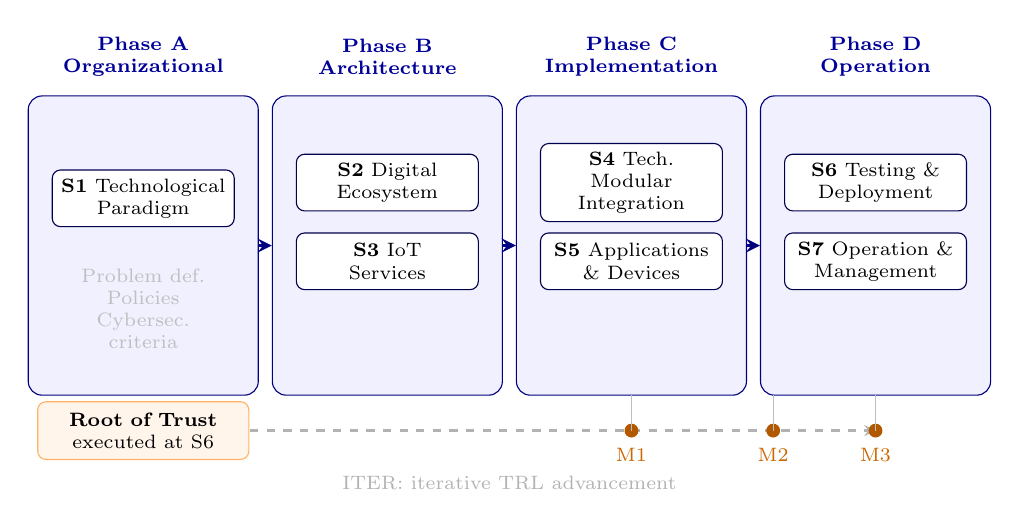
\begin{tikzpicture}[
  font=\small,
  every node/.style={},
  phbox/.style={
    draw=blue!50!black, fill=blue!6, rounded corners=5pt,
    minimum width=2.7cm, text width=2.5cm, minimum height=3.8cm,
    align=center, inner sep=6pt
  },
  phlabel/.style={
    font=\bfseries\scriptsize, text=blue!60!black,
    text width=2.4cm, align=center
  },
  stbox/.style={
    draw=blue!30!black, fill=white, rounded corners=3pt,
    minimum width=2.3cm, text width=2.1cm,
    minimum height=0.72cm, align=center,
    font=\scriptsize, inner sep=3pt
  },
  stno/.style={
    font=\bfseries\scriptsize, text=blue!70!black
  },
  flowarrow/.style={->, very thick, >=stealth, blue!50!black},
  iterarrow/.style={<->, thick, >=stealth, dashed, gray!60},
  maintpt/.style={circle, fill=orange!70!black, minimum size=5pt, inner sep=0}
]

% ── Phase A: Organizational ─────────────────────────────────
\node[phbox] (phA) at (0,0) {};
\node[phlabel] at (0, 2.4) {Phase A\\Organizational};
\node[stbox] at (0, 0.6) {\textbf{S1} Technological\\Paradigm};
\node[font=\scriptsize, text=gray!50, align=center, text width=2.1cm] at (0,-0.8) {Problem def. \\Policies\\Cybersec. criteria};

% ── Phase B: Architecture ───────────────────────────────────
\node[phbox] (phB) at (3.1,0) {};
\node[phlabel] at (3.1, 2.4) {Phase B\\Architecture};
\node[stbox] at (3.1, 0.8) {\textbf{S2} Digital\\Ecosystem};
\node[stbox] at (3.1,-0.2) {\textbf{S3} IoT\\Services};

% ── Phase C: Implementation ─────────────────────────────────
\node[phbox] (phC) at (6.2,0) {};
\node[phlabel] at (6.2, 2.4) {Phase C\\Implementation};
\node[stbox] at (6.2, 0.8) {\textbf{S4} Tech.\ Modular\\Integration};
\node[stbox] at (6.2,-0.2) {\textbf{S5} Applications\\\& Devices};

% ── Phase D: Operation ──────────────────────────────────────
\node[phbox] (phD) at (9.3,0) {};
\node[phlabel] at (9.3, 2.4) {Phase D\\Operation};
\node[stbox] at (9.3, 0.8) {\textbf{S6} Testing \&\\Deployment};
\node[stbox] at (9.3,-0.2) {\textbf{S7} Operation \&\\Management};

% ── Phase flow arrows ────────────────────────────────────────
\draw[flowarrow] (phA.east) -- (phB.west);
\draw[flowarrow] (phB.east) -- (phC.west);
\draw[flowarrow] (phC.east) -- (phD.west);

% ── ITER cycle arc ───────────────────────────────────────────
\draw[iterarrow] (0,-2.35) -- (9.3,-2.35)
    node[pos=0.5, below=0.45cm, font=\scriptsize, text=gray!60] {ITER: iterative TRL advancement};

% ── Maintenance points ───────────────────────────────────────
% M1 fires during implementation (Phase C, x=6.2)
\node[maintpt, label={[font=\scriptsize, text=orange!80!black]below:M1}] at (6.2,-2.35)  {};
% M2 fires during deployment (Phase D, x=8.0)
\node[maintpt, label={[font=\scriptsize, text=orange!80!black]below:M2}] at (8.0,-2.35)  {};
% M3 fires during operation (Phase D, x=9.3)
\node[maintpt, label={[font=\scriptsize, text=orange!80!black]below:M3}] at (9.3,-2.35)  {};

% ── Maintenance point tick lines ─────────────────────────────
\draw[thin, gray!50] (6.2,-1.9) -- (6.2,-2.35);
\draw[thin, gray!50] (8.0,-1.9) -- (8.0,-2.35);
\draw[thin, gray!50] (9.3,-1.9) -- (9.3,-2.35);

% ── RoT highlight note ──────────────────────────────────────
\node[draw=orange!60, fill=orange!8, rounded corners=3pt, font=\scriptsize,
      text width=2.4cm, align=center, inner sep=4pt] at (0,-2.35)
      {\textbf{Root of Trust}\\executed at S6};

\end{tikzpicture}

    \caption{Organization of the proposed methodology: four phases (Organizational, Architecture, Implementation, Operation) comprising seven numbered stages (S1--S7). Iterative development cycles (ITER) advance Technology Readiness Level. Maintenance points M1 (implementation), M2 (deployment), and M3 (operation) trigger targeted stage re-entry. The Root of Trust is executed at Stage~6.}
    \label{fig:metodologia}
\end{figure*}

\subsection{Phase A: Organizational (Stage~1)}

This phase addresses organizational considerations for IoT adoption. Stage~1 establishes the problem to be solved, operating policies, development policies, and cybersecurity criteria. The key processes are: problem definition with cost-benefit analysis (1.1); operating policies covering functional objectives, financial constraints, and regulatory compliance (1.2); development policies defining an iterative strategy using the TRL framework, timelines, and resource allocation (1.3); and cybersecurity policies covering criticality assessment, technological sovereignty, data sovereignty, supply chain security, and applicable government guidelines including Secure-by-Design \citep{ukgov2024sbdprinciples} and Privacy-by-Design \citep{enisa2017baseline} principles (1.4). Processes 1.4.2--1.4.3 operationalize the organizational-strategy layer of the sovereignty framework established in \citet{campos2026identity}, under which technological and data sovereignty are treated as emergent properties of who controls the entities' Root of Trust process rather than as external policy overlays.

\subsection{Phase B: Architecture (Stages~2--3)}

Stage~2 defines the IoT ecosystem architecture at the entity level: integration diagram, communication topology, entity hierarchy, functional processes, data flow, and scalability strategy. Critically, Stage~2 instantiates the formal identity model established in \citet{campos2026identity}, under which each entity $X$ in ecosystem $E$ possesses an identity:
\begin{equation}
    I^E_X = P^E_{X\;pub} \cup P^E_{X\;priv}
\end{equation}
where public parameters $P^E_{X\;pub}$ serve as identifiers and private parameters $P^E_{X\;priv}$ enable cryptographic operations, and authentication parameters $P^E_{X\;auth} \subset I^E_X$ and shared secrets $P^E_{X\;SS} \subset P^E_{X\;auth}$ are derived from this identity foundation (Figure~\ref{fig:identidad}). This methodology extends that model with an explicit cardinality count for each entity type $X$: the public-parameter and private-parameter counts are:
\begin{equation}
    n^E_X = |P^E_{X\;pub}|
\end{equation}
\begin{equation}
    k^E_X = |P^E_{X\;priv}|
\end{equation}
so that the total identity parameter count is $n^E_X + k^E_X$ and the table columns report the two component counts and their sum.

\begin{figure}[htbp]
    \centering
    % Figure: Identity parameter sets
% Nested rectangles: P_SS ⊆ P_auth ⊆ P_priv, with P_pub alongside.
% I^E_X = P_pub ∪ P_priv is the outer container.

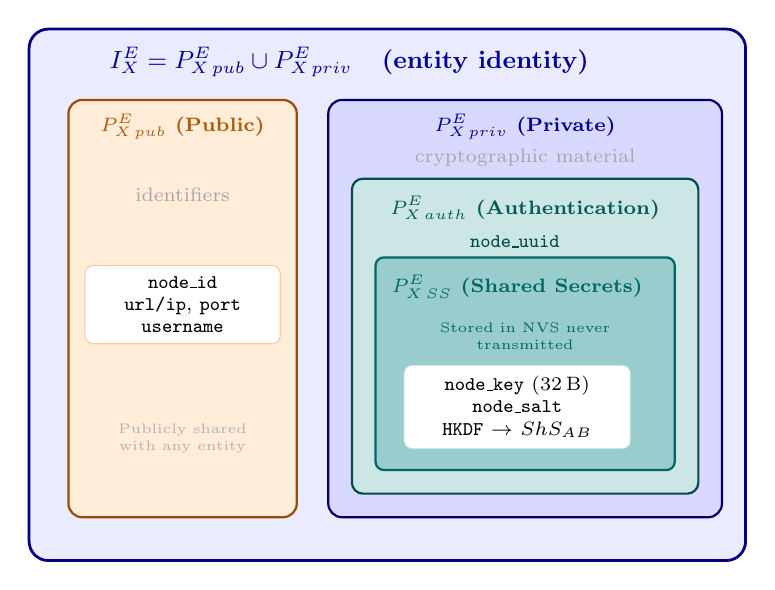
\begin{tikzpicture}[font=\small]

% ── Colour palette ──────────────────────────────────────────
\colorlet{outer}{blue!8}
\colorlet{priv}{blue!15}
\colorlet{auth}{teal!20}
\colorlet{ss}{teal!40}
\colorlet{pub}{orange!15}

% ── Outer identity box: I^E_X ────────────────────────────────
\draw[draw=blue!50!black, fill=outer, rounded corners=7pt, line width=1pt]
    (-0.3, -2.55) rectangle (8.8, 4.2);
\node[font=\bfseries\small, text=blue!60!black, anchor=north west]
    at (0.6, 4.1) {$I^E_X = P^E_{X\,pub} \cup P^E_{X\,priv}$\quad (entity identity)};

% ── P_pub box ───────────────────────────────────────────────
\draw[draw=orange!60!black, fill=pub, rounded corners=5pt, line width=0.8pt]
    (0.2, -2.0) rectangle (3.1, 3.3);
\node[font=\bfseries\scriptsize, text=orange!70!black, anchor=north]
    at (1.65, 3.25) {$P^E_{X\,pub}$ (Public)};
\node[font=\scriptsize, text=gray!70, anchor=north]
    at (1.65, 2.3) {identifiers};
\node[draw=orange!40, fill=white, rounded corners=3pt,
      font=\scriptsize, inner sep=4pt, text width=2.2cm, align=center]
    at (1.65, .7) {\texttt{node\_id}\\\texttt{url/ip}, \texttt{port}\\\texttt{username}};
\node[font=\tiny, text=gray!60, align=center, text width=2.4cm]
    at (1.65, -1.0) {Publicly shared\\with any entity};

% ── P_priv outer box ────────────────────────────────────────
\draw[draw=blue!40!black, fill=priv, rounded corners=5pt, line width=0.8pt]
    (3.5, -2.0) rectangle (8.5, 3.3);
\node[font=\bfseries\scriptsize, text=blue!60!black, anchor=north]
    at (6.0, 3.25) {$P^E_{X\,priv}$ (Private)};
\node[font=\scriptsize, text=gray!70, anchor=north]
    at (6.0, 2.8) {cryptographic material};

% ── P_auth inner box ────────────────────────────────────────
\draw[draw=teal!60!black, fill=auth, rounded corners=4pt, line width=0.8pt]
    (3.8, -1.7) rectangle (8.2, 2.3);
\node[font=\bfseries\scriptsize, text=teal!70!black, anchor=north]
    at (6.0, 2.2) {$P^E_{X\,auth}$ (Authentication)};

% ── P_SS innermost box ──────────────────────────────────────
\draw[draw=teal!80!black, fill=ss, rounded corners=3pt, line width=0.8pt]
    (4.1, -1.4) rectangle (7.9, 1.3);
\node[font=\bfseries\scriptsize, text=teal!80!black, anchor=north]
    at (5.9, 1.2) {$P^E_{X\,SS}$ (Shared Secrets)};
\node[draw=teal!30, fill=white, rounded corners=3pt,
      font=\scriptsize, inner sep=4pt, text width=2.6cm, align=center]
    at (5.9, -0.6) {\texttt{node\_key} (32\,B)\\\texttt{node\_salt}\\\texttt{HKDF} $\rightarrow$ $ShS_{AB}$};

% ── Non-SS auth params label ────────────────────────────────
\node[font=\scriptsize, text=teal!60!black, align=left, text width=1.4cm]
    at (6.0, 1.5) {\texttt{node\_uuid}};

% ── Containment annotations ─────────────────────────────────
\node[font=\tiny, text=teal!80!black, align=center, text width=5.0cm]
    at (6.0, 0.3) {Stored in NVS never\\ transmitted};

\end{tikzpicture}

    \caption{Identity parameter set hierarchy for entity $X$ in ecosystem $E$. Shared secrets $P_{SS}$ enable cryptographic operations; authentication parameters $P_{auth}$ prove identity; private parameters $P_{priv}$ are never disclosed; public parameters $P_{pub}$ serve as identifiers. In the SMG, the node's private identity parameter (its PUF response) lives in $P_{priv}$ but is never persisted to storage---only the non-secret mask/ECC helper data used to reconstruct it lives in ESP32~NVS, as $P_{pub}$.}
    \label{fig:identidad}
\end{figure}

Stage~3 specifies the services required for entity operation: secure storage subsystems, access control mechanisms, identity parameter storage strategies, and regulatory compliance integration. For constrained devices, Stage~3 requires an explicit cost/risk evaluation of persistent secure-storage options (hardware security modules, encrypted flash partitions) against physically-derived alternatives that avoid persisting a secret altogether; a Physically Unclonable Function (PUF) that regenerates the private identity parameter on demand from non-secret helper data is one such alternative, and its selection at Stage~4 is a direct consequence of this Stage~3 evaluation rather than an independent design choice. Servers and users retain conventional secrets management and MFA, respectively.

\subsection{Phase C: Implementation (Stages~4--5)}

Stage~4 selects enabling technologies aligned with policies from Stage~1 and architecture from Stages~2--3. Technology choices are evaluated against maturity level (TRL), vulnerability landscape, and supply chain risk. For the SMG, Stage~4 selects \texttt{esp32\_puflib} \citep{stanicek2022esp32puflib}, an SRAM-based PUF implementation for the ESP32 family, as the identity-generation mechanism motivated by the Stage~3 secure-storage evaluation above. Because \texttt{esp32\_puflib} is implemented as a native C/ESP-IDF component, Stage~4 also selects a C/ESP-IDF firmware architecture for the node---rather than the MicroPython runtime used in the prior PSK+NVS instantiation---so that the PUF library is linked directly, without a language-runtime wrapper; the same decision replaces the previous MicroPython \texttt{aesgcm} companion module with ESP-IDF's native \texttt{mbedtls}/\texttt{esp\_aes} AES-256-GCM support. This platform choice is itself a direct, traceable consequence of the Stage~3 evaluation, not an independent implementation preference. Stage~5 implements all ecosystem elements: servers, devices, databases, communication infrastructure, IoT services, and applications. Security is enforced through secure coding practices, unit testing of security mechanisms, and validation against applicable security guidelines (Secure-by-Design principles \citep{ukgov2024sbdprinciples}, NIST IoT Cybersecurity Guidance \citep{NIST_IoT_2020}, and OWASP IoT Top~10).

\subsection{Phase D: Operation (Stages~6--7)}

Stage~6 covers deployment, configuration, and testing: individual component validation, infrastructure deployment, \emph{Root of Trust execution} for all entities (Process~6.1.3), general operation verification, and security testing (penetration testing at higher TRLs; tamper verification at TRL~3). Stage~7 addresses ongoing operation: monitoring, element maintenance, information lifecycle management, threat intelligence, element updates, incident response, and network infrastructure oversight.

\subsection{Iterative Development and Maintenance}

The methodology supports iterative advancement through TRL-guided cycles (ITER) and three structured maintenance points: M1 (during implementation, triggers technology re-evaluation), M2 (during deployment, triggers code revision), and M3 (during operation, triggers architectural redesign). M1 fires when an implementation-phase review reveals that the chosen technology cannot satisfy a stage requirement; M2 fires when deployment-phase testing reveals that the implementation requires code-level revision to meet a security or functional requirement; M3 fires when operation-phase monitoring reveals that the deployed architecture cannot accommodate an observed operational pattern. This structure supports progressive maturation from proof-of-concept to production deployment.

\subsection{Root of Trust Establishment}

Building on the four-phase Root of Trust process of \citet{campos2026identity}, we instantiate its parameter generation, secure storage, exchange, and peer-management phases as concrete protocol message sequences for both cryptographic schemes.

\textbf{Symmetric scheme (resource-constrained devices):} Rather than generating a random device key and persisting it in flash, the device's identity key is derived on demand from a Physically Unclonable Function (PUF), instantiated via \texttt{esp32\_puflib} \citep{stanicek2022esp32puflib}. \emph{Enrollment} (performed once, Table~\ref{tab:rotpsim}) reads the ESP32's RTC~FAST~SRAM power-up state across repeated measurements and derives two non-secret artifacts---a stable-bit mask and error-correction (helper) data---that are stored on the device and allow the same physical response to be reconstructed, with correction, on every subsequent boot; neither artifact discloses the response without physical access to the specific chip. During the same enrollment, the device computes a one-way verifier of its response and registers it with the server; the server's own verifier (its identity counterpart, not PUF-derived---see below) is pinned on the device. \emph{Session identification} (Table~\ref{tab:rotpsim_b}) is a \emph{cryptographic hash-reconstruction challenge}: each side issues the other a fresh random nonce, reconstructs its own verifier (the device physically, via the PUF; the server from conventional storage), and proves fresh knowledge of it by hashing it together with the peer's nonce---never transmitting the verifier or the underlying response itself, and never reusing a prior proof, since each is bound to a nonce that changes every session. Parameters are stored securely (Table~\ref{tab:rotpsim}); critically, the device persists no secret of its own: the only values written to its NVS are the non-secret stable-bit mask and ECC helper data (both classified $P_{pub}$) and the pinned server verifier $V_B$, which serves as the device's trust anchor for server authentication. The node's own private identity parameter ($\text{PUF}_A$, and hence its verifier $V_A$) exists only transiently in RAM during each boot and is never written to storage (Section~\ref{sec:conceptual}).

\textbf{Server identity:} the server is not a good physical candidate for PUF-based identity (no comparable unclonable analog substrate is assumed for the RPi4), so its identity parameter is a conventionally-provisioned, equivalent counterpart in the same formal role: a value provisioned on the server and pinned on each enrolled device as that device's server-authentication trust anchor. Because the scheme is symmetric, possession of $V_B$ is exactly what the server must prove per session, via the same nonce-bound hash-reconstruction challenge the device applies to its own $V_A$; equivalently, $V_B$ functions as the pairwise shared secret for server authentication, and its confidentiality on the device side is bounded by the device's physical security (see the Information Disclosure row in Table~\ref{tab:stride_b} and the Limitations). This keeps both entities' identity parameters structurally symmetric in the model of \citet{campos2026identity} ($I^E_X = P^E_{X\,pub} \cup P^E_{X\,priv}$) while acknowledging that only the constrained device benefits from a physically-unclonable generation mechanism.

\textbf{Asymmetric scheme (capable devices):} Entities generate public/private key pairs, exchange public keys with identifiers, and store the peer's public key for subsequent authentication using ISO/IEC~9798-3 mutual authentication \citep{isoiec9798} (Table~\ref{tab:rotpasym}).

\begin{table}[htbp]
    \centering
    \caption{Root of Trust process: PUF-based symmetric key establishment --- Phase 1 (enrollment and mutual verifier registration, performed once, over an isolated/physical provisioning channel). $\text{PUF}_A$ denotes the device's PUF response, reconstructed from RTC~FAST~SRAM via \texttt{esp32\_puflib}; \texttt{mask}$_A$/\texttt{ecc}$_A$ are the non-secret stable-bit mask and error-correction helper data. $V_B$ is the server's conventionally-provisioned identity counterpart (Section~\ref{sec:methodology}, ``Server identity''), not PUF-derived.}
    \label{tab:rotpsim}
    \small
    \begin{tabular}{
        >{\centering\arraybackslash}p{3.8cm}
        c
        >{\centering\arraybackslash}p{4.0cm}
        c
        >{\centering\arraybackslash}p{3.8cm}
    }
        \toprule
        \textbf{Device} & & \textbf{Message} & & \textbf{Server} \\
        \midrule
        $\{ID_A,\;MAC_A\}$ enroll\_puf() $\rightarrow \{\text{mask}_A,\;\text{ecc}_A\}$ (stored, public) & & & & $\{ID_B,\;URL/IP_B,\;Port_B\}$; $V_B$ provisioned (stored) \\
        get\_puf\_response() $\rightarrow \text{PUF}_A$; $V_A \leftarrow \text{SHA-256}(\text{PUF}_A)$ & & & & \\
        & & $\{ID_A,\;MAC_A,\;V_A\}$ ${\rightarrow}$ & & \\
        & & ${\leftarrow}$ $\{ID_B,\;URL/IP_B,$ $Port_B,\;V_B\}$ & & \\
        pin (store): $\{ID_B,\;V_B\}$ as server reference & & & & store verifier: $\{ID_A,\;V_A\}$ as device reference (not $\text{PUF}_A$ itself) \\
        \bottomrule
    \end{tabular}
\end{table}

\begin{table}[htbp]
    \centering
    \caption{Root of Trust process: PUF-based symmetric key establishment --- Phase 2 (per-boot reconstruction and nonce-bound hash-reconstruction challenge; continues Table~\ref{tab:rotpsim}). $V_A$ is never transmitted after Phase~1---each side proves fresh knowledge of its own reconstructed verifier by hashing it with a nonce supplied by the peer. No secret is persisted on the device between Phase~1 and Phase~2; $\text{PUF}_A$ is regenerated each time.}
    \label{tab:rotpsim_b}
    \small
    \begin{tabular}{
        >{\centering\arraybackslash}p{3.8cm}
        c
        >{\centering\arraybackslash}p{4.0cm}
        c
        >{\centering\arraybackslash}p{3.8cm}
    }
        \toprule
        \textbf{Device} & & \textbf{Message} & & \textbf{Server} \\
        \midrule
        generate nonce $N_A$ & & $\{ID_A,\;N_A\}$ ${\rightarrow}$ & & generate nonce $N_B$ \\
        get\_puf\_response() using $\{\text{mask}_A,\;\text{ecc}_A\}$ $\rightarrow \text{PUF}_A$; $V_A \leftarrow \text{SHA-256}(\text{PUF}_A)$ & & ${\leftarrow}$ $\{ID_B,\;N_B,\;R_B = \text{SHA-256}(V_B \!\parallel\! N_A)\}$ & & compute $R_B$ from stored $V_B$ \\
        verify $R_B \stackrel{?}{=} \text{SHA-256}(V_B \!\parallel\! N_A)$ using pinned $V_B$ (server authentication); $R_A \leftarrow \text{SHA-256}(V_A \!\parallel\! N_B)$ & & $\{R_A\}$ ${\rightarrow}$ & & verify $R_A \stackrel{?}{=} \text{SHA-256}(V_A \!\parallel\! N_B)$ using stored reference $V_A$ (device identification) \\
        & & ${\leftarrow}$ $\{\text{session\_ack}\}$ (or rejection if verification failed) & & issue \texttt{session\_ack} only if $R_A$ verified \\
        $\text{SHA-256}(V_A \!\parallel\! V_B \!\parallel\! N_A \!\parallel\! N_B)$ ${\rightarrow Key_{ab}}$ & & & & $\text{SHA-256}(V_A \!\parallel\! V_B \!\parallel\! N_A \!\parallel\! N_B)$ ${\rightarrow Key_{ab}}$ \\
        $Key_{ab}$ held only in RAM for session duration; no on-device secure store required & & & & $Key_{ab}$ held in RAM; $V_A$ reference retained in server storage \\
        \bottomrule
    \end{tabular}
\end{table}
\noindent\textit{Implementation note:} the PUF-based implementation source (\texttt{smg\_puf\_rot\_node/}, device side; \texttt{smg\_primary\_server/rot\_challenge\_service.py}, server side; companion code repository, Materials Availability) uses \texttt{ShS\_A}/\texttt{ShS\_B} for $V_A$/$V_B$, \texttt{challenge\_a}/\texttt{challenge\_b} for $N_A$/$N_B$, and \texttt{server\_proof}/\texttt{device\_proof} for $R_B$/$R_A$; the four-message sequence and the $Key_{ab}$ derivation above match the implementation exactly, including concatenation order, verified directly against the source on 2026-10-05.

\begin{table}[htbp]
    \centering
    \caption{Root of Trust process: asymmetric key establishment.}
    \label{tab:rotpasym}
    \small
    \begin{tabular}{
        >{\centering\arraybackslash}p{3.8cm}
        c
        >{\centering\arraybackslash}p{4.0cm}
        c
        >{\centering\arraybackslash}p{3.8cm}
    }
        \toprule
        \textbf{Device} & & \textbf{Message} & & \textbf{Server} \\
        \midrule
        $\{ID_A,\;MAC_A,$ $PubKey_A,\;PrivKey_A\}$ & & & & $\{ID_B,\;URL/IP_B,$ $Port_B,\;PubKey_B,$ $PrivKey_B\}$ \\
        & & $\{ID_A,\;MAC_A,\;PubKey_A\}$ ${\rightarrow}$ & & \\
        & & ${\leftarrow}$ $\{ID_B,\;URL/IP_B,$ $Port_B,\;PubKey_B\}$ & & \\
        secure store: $\{PubKey_B,$ $ID_B,\;URL/IP_B,\;Port_B\}$ & & & & secure store: $\{PubKey_A,\;ID_A,\;MAC_A\}$ \\
        \bottomrule
    \end{tabular}
\end{table}

\subsection{Threat Coverage by Design: STRIDE Analysis}
\label{subsec:stride}

We analyze how the methodology's stages address the STRIDE (Spoofing, Tampering, Repudiation, Information Disclosure, Denial of Service, and Elevation of Privilege) threat categories \citep{shostack2014threat} for centralized IoT ecosystems. Unlike framework-specific threat models tied to particular technologies, this analysis maps threats to methodology stages and technology-agnostic mechanism categories, ensuring applicability across implementations.

Tables~\ref{tab:stride_a} and~\ref{tab:stride_b} map each STRIDE threat to the methodology stage(s) providing countermeasures, the mechanism category mandated by those stages, and the instantiation in the SMG case study. The adversary $\mathcal{A}$ is assumed to have network access, commodity computational resources, and knowledge of the system architecture (Kerckhoffs's principle); goals include unauthorized data access, service disruption, entity impersonation, and credential exfiltration.

\begin{table*}[htbp]
    \centering
    \caption{STRIDE threat model: mapping to methodology stages and SMG instantiation --- Part 1 (Spoofing, Tampering, Repudiation).}
    \label{tab:stride_a}
    \small
    \renewcommand{\arraystretch}{1.2}
    \begin{tabular}{
        >{\raggedright\arraybackslash}p{2.3cm}
        >{\raggedright\arraybackslash}p{2.3cm}
        >{\raggedright\arraybackslash}p{2.4cm}
        >{\raggedright\arraybackslash}p{3.0cm}
        >{\raggedright\arraybackslash}p{3.0cm}
        >{\centering\arraybackslash}p{1.6cm}
    }
        \toprule
        \textbf{Threat} & \textbf{Attack Vector} & \textbf{Methodology Stage(s)} & \textbf{Mechanism Category} & \textbf{SMG Instantiation} & \textbf{Residual Risk} \\
        \midrule
        \textbf{Spoofing} & Entity impersonation; forged credentials & 2.2.2 (auth mech.), 2.2.3 (RoT), 6.1.3 (RoT execution) & Cryptographic mutual authentication using entity-specific, PUF-derived identity commitments & PUF-derived identity (\texttt{esp32\_puflib}) + nonce-bound SHA-256 hash-reconstruction challenge; no persistent secret in NVS; mutual handshake before any data accepted; bidirectional mutual authentication confirmed in 30/30 real hard-reset trials on SMG\_NODE\_01 (Section~\ref{subsec:pufbench}) & Low (requires physical device compromise) \\
        \midrule
        \textbf{Tampering} & Data modification in transit; sensor reading manipulation & 2.2.4 (secure comms), 5.2.1 (secure dev.) & Authenticated encryption with integrity binding per message; random nonces & AES-256-GCM per message; 12-byte random nonce per message; the GCM authentication tag detects any single-message modification & Low for per-message tampering (GCM tag); Medium for message reordering/replay within a session (no message-sequence chain in this design, see Limitations) \\
        \midrule
        \textbf{Repudiation} & Denial of sent data; dispute of control commands & 2.2.2 (session audit), 3.1 (data service), 7.1 (monitoring) & Session-bound data exchange with server-side session logging & Server logs each authenticated session under \texttt{node\_id} and timestamp (Stage~7.1); coverage is evidentiary (log-based), not an independently-verifiable cryptographic chain (design trade-off, see Limitations) & Medium (logs can be disputed without independent cryptographic chain verification) \\
        \bottomrule
    \end{tabular}
\end{table*}

\begin{table*}[htbp]
    \centering
    \caption{STRIDE threat model (continued from Table~\ref{tab:stride_a}) --- Part 2 (Information Disclosure, Denial of Service, Elevation of Privilege).}
    \label{tab:stride_b}
    \small
    \renewcommand{\arraystretch}{1.2}
    \begin{tabular}{
        >{\raggedright\arraybackslash}p{2.3cm}
        >{\raggedright\arraybackslash}p{2.3cm}
        >{\raggedright\arraybackslash}p{2.4cm}
        >{\raggedright\arraybackslash}p{3.0cm}
        >{\raggedright\arraybackslash}p{3.0cm}
        >{\centering\arraybackslash}p{1.6cm}
    }
        \toprule
        \textbf{Threat} & \textbf{Attack Vector} & \textbf{Methodology Stage(s)} & \textbf{Mechanism Category} & \textbf{SMG Instantiation} & \textbf{Residual Risk} \\
        \midrule
        \textbf{Information Disclosure} & Key extraction; credential exfiltration; traffic interception & 1.4.2--1.4.3 (sovereignty), 2.2.1 (identity params), 5.2.1 (secure dev.) & Data sovereignty policy; no persistent device-own secret to disclose; application-layer encryption & The node's private parameter is reconstructed at boot from the PUF (\texttt{esp32\_puflib}) and never persisted: only non-secret mask/ECC helper data is written to NVS, plus the pinned server verifier $V_B$ (trust anchor); all data AES-256-GCM encrypted in transit & Node identity: Low (no node secret exists at rest; forging $V_A$ requires the enrolled chip's physical response or the server's stored verifier). Server impersonation from a captured unit: Medium ($V_B$ is readable from that unit's NVS; the centralized single-primary topology contains the exposure --- see Limitations) \\
        \midrule
        \textbf{Denial of Service} & Authentication flooding; bus load disruption; node isolation & 7.1 (monitoring), 7.2.1 (anomaly detect.), 2.1.8 (hierarchy) & Anomaly-based trust scoring; degraded-mode operation; entity isolation policy & Trust score decay on repeated failures; UNTRUSTED nodes isolated (TCP dropped); last PWM duty maintained on timeout & Medium (physical-layer DoS outside software scope) \\
        \midrule
        \textbf{Elevation of Privilege} & Node masquerading as admin; unauthorized config access & 2.1.8 (entity hierarchy), 3.2.1 (access control), 2.2.2 (auth) & Entity type hierarchy with API-enforced access control; token type includes entity class & Node session tokens permit only POST sensor data; admin endpoints reject non-admin tokens & Low (token type embedded in authenticated session) \\
        \bottomrule
    \end{tabular}
\end{table*}


% ============================================================
\section{Case Study: DC Smart Microgrid IoT Ecosystem}
\label{sec:casestudy}
% ============================================================

\subsection{Case Study Design}

This case study follows a \textbf{confirmatory design} \citep{yin2014case}: the methodology constitutes the theoretical proposition; the SMG implementation constitutes the empirical test. Evidence is collected from four sources following Yin's principle of multiple evidence sources (Table~\ref{tab:datasources}).

\begin{table}[htbp]
    \centering
    \caption{Data collection protocol: evidence sources.}
    \label{tab:datasources}
    \small
    \renewcommand{\arraystretch}{1.15}
    \begin{tabular}{
        >{\raggedright\arraybackslash}p{2.8cm}
        >{\raggedright\arraybackslash}p{2.4cm}
        >{\raggedright\arraybackslash}p{7.0cm}
    }
        \toprule
        \textbf{Source} & \textbf{Evidence Type} & \textbf{Content} \\
        \midrule
        Design documents & Documentary & Stage outputs: policies, architecture diagrams, identity tables, service specifications \\
        Firmware artifacts & Physical artifact & ESP32 C/ESP-IDF modules: sensor reading, EMS, identity (PUF enrollment/reconstruction, \texttt{esp32\_puflib}), communication (AES-256-GCM), metrics \\
        Execution logs & Archival records & Authentication logs, RoT deployment logs, functional test reports, \texttt{/methodology.csv} output \\
        Measurements & Quantitative & Handshake latency, sampling rate, payload size, heap stability, OWASP coverage \\
        \bottomrule
    \end{tabular}
\end{table}

\subsection{Research Questions}

\begin{table}[htbp]
    \centering
    \caption{Case study research questions.}
    \label{tab:csq}
    \small
    \renewcommand{\arraystretch}{1.15}
    \begin{tabular}{
        >{\centering\arraybackslash}p{0.9cm}
        >{\raggedright\arraybackslash}p{6.0cm}
        >{\raggedright\arraybackslash}p{5.0cm}
    }
        \toprule
        \textbf{ID} & \textbf{Question} & \textbf{Addressed by} \\
        \midrule
        CSQ1 & Does the methodology provide sufficient guidance to architect a complete, secure IoT ecosystem for a real industrial application? & Stage-by-stage traceability; completeness of outputs; functional test results \\
        CSQ2 & Does the parameterized identity model enable unambiguous security mechanism definition across heterogeneous entity types? & Identity parameter table; authentication implementation; coverage across 4 entity types \\
        CSQ3 & Does the Root of Trust Process establish verifiable secure communication between ecosystem entities? & RoT execution evidence; handshake latency measurements; mutual challenge-response verification \\
        CSQ4 & What is the methodology's coverage of known IoT security threats relative to established standards? & OWASP IoT Top~10 mapping; security mechanism traceability \\
        \bottomrule
    \end{tabular}
\end{table}

\subsection{Case Context}

%% REDLINE C3: "geographically separated" -> "co-located laboratory" (factual; nodes are co-located in a controlled lab per phase3_plan.md §5c)
\textbf{Application domain:} The SMG manages distributed DC electrical energy generation, storage, and consumption across two co-located nodes in a controlled laboratory environment. The growing integration of renewable energy sources (solar panels, batteries) into local grids requires intelligent, automated management to balance generation and demand in real time without relying on centralized national grid infrastructure. This application is classified as critical infrastructure (Methodology Stage~1, Process~1.4.1), requiring the highest cybersecurity tier.

\textbf{Physical architecture:} The SMG consists of two secondary control agent nodes and one primary agent (Raspberry Pi~4B). Each secondary node connects a renewable generation element to a shared 12\,V DC bus with local energy storage (Table~\ref{tab:hardware}). The primary agent runs on a Raspberry Pi~4B connected to the DC bus as a pure load via a DC/AC inverter ($12\,\text{V DC} \rightarrow 120\,\text{V AC}$) followed by a USB-C AC/DC adapter.

\begin{table}[htbp]
    \centering
    \caption{Secondary node hardware components.}
    \label{tab:hardware}
    \small
    \renewcommand{\arraystretch}{1.15}
    \begin{tabular}{
        >{\raggedright\arraybackslash}p{3.5cm}
        >{\raggedright\arraybackslash}p{3.2cm}
        >{\raggedright\arraybackslash}p{7.5cm}
    }
        \toprule
        \textbf{Component} & \textbf{Role} & \textbf{Specification} \\
        \midrule
        ESP32 NodeMCU & IoT + EMS controller & Dual-core 240\,MHz, 520\,KB SRAM, 4\,MB Flash, built-in WiFi; powered by local battery via DC-DC buck (12V→5V) \\
        Epcom AGM VRLA & Local energy storage + ESP32 supply & PL-18-12, 12\,V, 18\,Ah; also supplies ESP32 via buck converter \\
        IBFIA DC-DC SSR $\times$3 & Energy flow control & 3--32\,VDC control, 5--60\,VDC load, 40\,A; driven by ESP32 LEDC on GPIO27/26/25 at 1\,kHz, 10-bit \\
        Schneider MCB $\times$3 & Overcurrent protection & 2-pole, one per SSR channel \\
        Solar charge controller & Energy flow control & Commercial MPPT controller (handles droop control and battery-charging voltage regulation autonomously) \\
        ACS712-05B $\times$2 & Current sensing & Hall-effect, 185\,mV/A, 16-sample median oversampling \\
        Resistive divider $\times$2 & Voltage sensing & 30\,k$\Omega$/7.5\,k$\Omega$ (5:1 ratio); reads up to 16.5\,V on 3.3\,V ADC \\
        \bottomrule
    \end{tabular}
\end{table}

\textbf{Digital architecture:} The ecosystem uses a centralized communication topology (Stage~2.1.4) with fog processing (Stage~2.1.7): each ESP32 executes local sensor fusion and a 9-rule fuzzy Energy Management System (EMS), while the RPi4 runs global coordination with a 27-rule security-aware EMS. The entity hierarchy is: IoT Nodes (lowest privilege) $<$ Users $<$ Administrators. Development target: TRL~3 (proof of concept with physical elements).

\subsection{Stage-by-Stage Traceability}

Tables~\ref{tab:traceability_a} and~\ref{tab:traceability_b} document the application of each methodology stage to the SMG, showing the decision made at each stage and the measurable artifact produced. This traceability table constitutes the primary evidence for CSQ1.

\begin{table*}[htbp]
    \centering
    \caption{Stage-by-stage traceability: methodology process $\rightarrow$ SMG decision $\rightarrow$ artifact --- Part 1 (Stages 1--3).}
    \label{tab:traceability_a}
    \small
    \renewcommand{\arraystretch}{1.0}
    \begin{tabular}{
        >{\centering\arraybackslash}p{1.5cm}
        >{\raggedright\arraybackslash}p{3.2cm}
        >{\raggedright\arraybackslash}p{4.8cm}
        >{\raggedright\arraybackslash}p{4.0cm}
    }
        \toprule
        \textbf{Stage} & \textbf{Methodology Process} & \textbf{Decision Made in SMG} & \textbf{Artifact} \\
        \midrule
        \multirow{4}{=}{\textbf{1} Technological Paradigm}
            & 1.1 Establish problem & Manage distributed renewable energy nodes securely in a 12\,V DC microgrid & Problem specification \\
            & 1.1.2 Entities involved & 5 entity types: IoT nodes, server, users, admins, DC bus & Entity list \\
            & 1.4.1 Criticality & Classified as critical infrastructure (electrical energy) & High-security cybersecurity policy \\
            & 1.4.2 Technological sovereignty & Self-hosted; no third-party cloud; ESP32 + local RPi4 server & Architecture constraint record \\
            & \multicolumn{3}{p{12.6cm}}{\scriptsize\textit{Of the seven conceptual-framework element types (Section~\ref{sec:conceptual}), the SMG instantiates five: storage/communication infrastructure are subsumed into the server, and IoT services into the device/server software. Of the five entity types, four (nodes, server, users, admins) carry digital identity (Table~\ref{tab:identity}); the DC bus is tracked via P3 sensor-data integrity instead.}} \\
        \midrule
        \multirow{5}{=}{\textbf{2} Digital Ecosystem}
            & 2.1.4 Communication topology & Centralized: all nodes report to primary agent & Architecture diagram \\
            & 2.1.7 Processing topology & Fog: local EMS on ESP32; global coordination on RPi4 & Processing topology record \\
            & 2.2.1 Identity definition & 4 entity types, 14 identity parameters total (non-uniform per type; Table~\ref{tab:identity}) & Identity parameter table \\
            & 2.2.2 Authentication mechanism & Nonce-bound SHA-256 hash-reconstruction challenge (PUF-derived device identity, conventionally-provisioned equivalent server identifier); AES-256-GCM session encryption & Authentication diagram \\
            & 2.2.3 Root of Trust process & 4-phase RoT designed for node--server pairs & RoT execution log \\
        \midrule
        \multirow{2}{=}{\textbf{3} IoT Services}
            & 3.1 Service definition & 4 services: data ingestion, EMS coordination, auth API, monitoring & Service specification \\
            & 3.2.1 Access control & Token-based; nodes: POST only; users: GET; admins: full & Access control matrix \\
        \bottomrule
    \end{tabular}
\end{table*}

\begin{table*}[htbp]
    \centering
    \caption{Stage-by-stage traceability (continued from Table~\ref{tab:traceability_a}) --- Part 2 (Stages 4--7).}
    \label{tab:traceability_b}
    \small
    \renewcommand{\arraystretch}{0.95}
    \begin{tabular}{
        >{\centering\arraybackslash}p{1.5cm}
        >{\raggedright\arraybackslash}p{3.2cm}
        >{\raggedright\arraybackslash}p{4.8cm}
        >{\raggedright\arraybackslash}p{4.0cm}
    }
        \toprule
        \textbf{Stage} & \textbf{Methodology Process} & \textbf{Decision Made in SMG} & \textbf{Artifact} \\
        \midrule
        \multirow{4}{=}{\textbf{4} Tech.\ Modular Integration}
            & 4.1.1 TRL planning & TRL~3 target for ITER~1; laboratory proof of concept & TRL milestone record \\
            & 4.1.2 Platform selection & ESP32 + C/ESP-IDF: WiFi built-in, SHA-256 HW, NVS, \texttt{esp32\_puflib} linked as a native ESP-IDF component & Technology selection rationale \\
            & 4.1.3 Communication & WiFi IEEE~802.11\,b/g/n + TCP; application-layer hash-reconstruction challenge protocol (\texttt{rot\_session.c}/\texttt{rot\_challenge\_service.py}) & Protocol selection record \\
            & 4.2 Vulnerability mitigation & ESP-IDF v5.4.2 pinned (per the flashed firmware build log); nonce reuse fixed & Risk register \\
        \midrule
        \multirow{3}{=}{\textbf{5} Applications \& Devices}
            & 5.1.1 Server & REST API + time-series database + monitoring dashboard on RPi4 & Server deployment \\
            & 5.1.2 Devices & ESP32 C/ESP-IDF firmware (\texttt{smg\_puf\_rot\_node}): identity (PUF), Root of Trust, and secure-communication modules; sensor/EMS modules not yet re-ported from the prior MicroPython firmware (see Limitations) & Firmware artifact \\
            & 5.2.1 Secure development & NVS stores only non-secret mask/ECC helper data (no persistent secret); \texttt{esp\_fill\_random()} nonces (ESP-IDF hardware RNG); no credentials in source & Code review record \\
        \midrule
        \multirow{3}{=}{\textbf{6} Testing \& Deployment}
            & 6.1.3 RoT execution & Prior PSK+NVS scheme: RoT executed for all 2 nodes at deployment (100\%); PUF-based redesign: executed and validated on 1/2 nodes (SMG\_NODE\_01; SMG\_NODE\_02 pending, Section~\ref{subsec:pufbench}) & Deployment log (2 entries); PUF bench (Section~\ref{subsec:pufbench}) \\
            & 6.2.1 Functional testing & 8 functional tests: boot, identity, auth, fuzzy EMS, saturation — all pass & Test report (8/8 pass) \\
            %% REDLINE M6: relabel "Penetration testing" as "Tamper verification" (single negative test, not a pen test)
            & 6.2.2 Tamper verification & NVS parameter tampering confirmed as authentication failure (single targeted negative test; full penetration testing deferred to ITER~2) & Security verification log \\
        \midrule
        \multirow{2}{=}{\textbf{7} Operation \& Mgt.}
            & 7.1.1 Monitoring & Real-time V, I, P, PWM duty per node; authentication status; session history & Dashboard artifact \\
            & 7.2.2 Update elements & OTA update policy defined with authentication requirement (ITER~2 target) & Update policy \\
        \bottomrule
    \end{tabular}
\end{table*}

\subsection{Identity Parameter Definition (Stage~2.2.1)}

Applying Equations~(1)--(3) to the SMG entities produces a 14-parameter identity model (Table~\ref{tab:identity}). The public/private/authentication parameter separation directly determined the authentication mechanism (PUF-derived commitment using the private, non-persistent parameter) and the secure storage requirement for the IoT Node: none, beyond the non-secret mask/ECC helper data already classified as public.
%% PENDING-PUF-DATA: parameter counts below reflect the PUF-based redesign; re-verify against the actual esp32_puflib integration once implemented.

\begin{table}[htbp]
    \centering
    \caption{Identity parameter table: Stage~2.2.1 output for the SMG. \texttt{mask}$_A$/\texttt{ecc}$_A$: non-secret stable-bit mask and error-correction helper data generated at enrollment by \texttt{esp32\_puflib}, stored in ESP32 NVS. PUF response$^\dagger$: the device's physically-derived private identity parameter, reconstructed from \texttt{mask}$_A$/\texttt{ecc}$_A$ on every boot and never persisted (see note below). Following Eqs.~(2)--(3), $n = n^E_X$ is the public-parameter count, $k = k^E_X$ the private-parameter count, and Total $= n^E_X + k^E_X$ the total identity-parameter count.}
    \label{tab:identity}
    \small
    \renewcommand{\arraystretch}{1.2}
    \begin{tabular}{
        >{\raggedright\arraybackslash}p{2.0cm}
        >{\centering\arraybackslash}p{1.5cm}
        >{\raggedright\arraybackslash}p{2.4cm}
        >{\raggedright\arraybackslash}p{2.4cm}
        >{\raggedright\arraybackslash}p{2.4cm}
        >{\centering\arraybackslash}p{0.6cm}
        >{\centering\arraybackslash}p{0.6cm}
        >{\centering\arraybackslash}p{0.6cm}
    }
        \toprule
        \textbf{Entity Type} & \textbf{Class} & $P_{pub}$ & $P_{priv}$ & $P_{auth}$ & $n$ & $k$ & \textbf{Total} \\
        \midrule
        IoT Node (ESP32) & Device & \texttt{node\_id}, \texttt{mask}$_A$, \texttt{ecc}$_A$ & \texttt{node\_uuid}, PUF response$^\dagger$ & \texttt{node\_uuid}, PUF response$^\dagger$ & 3 & 2 & 5 \\
        IoT Server (RPi4) & Server & \texttt{url/ip}, \texttt{port} & \texttt{server\_uuid} & \texttt{server\_uuid} & 2 & 1 & 3 \\
        User & User & \texttt{username} & \texttt{user\_uuid}, \texttt{password} & \texttt{user\_uuid}, \texttt{password} & 1 & 2 & 3 \\
        Administrator & Admin & \texttt{username} & \texttt{admin\_uuid}, \texttt{password} & \texttt{admin\_uuid}, \texttt{password} & 1 & 2 & 3 \\
        \midrule
        \textbf{Total} & & \textbf{7} & \textbf{7} & \textbf{7} & & & \textbf{14} \\
        \bottomrule
    \end{tabular}
\end{table}

The entity-specific separation of identity parameters produced a direct, unambiguous mapping to implementation artifacts: \texttt{node\_id}, \texttt{node\_uuid}, \texttt{mask}$_A$, and \texttt{ecc}$_A$ correspond to distinct NVS keys written at enrollment time; no parameter redefinition or additional design decisions were required at the specification level. In the present case study, $P_{auth}$ and $P_{priv}$ coincide for every entity type (all private parameters participate in authentication, as shown in Table~\ref{tab:identity}); this is a case-study-specific coincidence, not a general property of the model---\citet{campos2026identity} define only the broader relation $P_{auth} \subset I$ (Figure~\ref{fig:identidad}), so future case studies may include a private parameter not used for authentication (e.g., a long-term audit key), in which case $P_{auth} \subsetneq P_{priv}$ rather than $P_{auth} = P_{priv}$.

$^\dagger$\textbf{Note on the PUF response as a non-persistent private parameter:} the formal identity model $I^E_X = P^E_{X\;pub} \cup P^E_{X\;priv}$ (Section~\ref{sec:methodology}) classifies a parameter as private or public by its confidentiality role, not by whether it is stored. The IoT Node's PUF response satisfies $P_{priv}$'s role---it is never disclosed and underlies the device's authentication proof---while never existing as data at rest: it is regenerated from \texttt{mask}$_A$/\texttt{ecc}$_A$ (both $P_{pub}$) on every boot. This is the concrete instance of the Phase~2 (secure storage) trivialization noted in Section~\ref{sec:conceptual}.

\subsection{Security Mechanism Analysis: STRIDE--to--Protocol Mapping}
\label{subsec:strideprot}

The methodology-level STRIDE analysis (Section~\ref{subsec:stride}) identifies mechanism categories that address each threat category at the framework level, independent of implementation technology. This subsection demonstrates how the SMG's Stage~4 technology selection instantiates those mechanisms through three authentication and data-exchange protocol phases (P1--P3), establishing a complete traceability chain from threat identification to deployed countermeasure.

\textbf{Scope note:} Phases P1--P3 constitute an \emph{implementation-specific} Stage~4 technology choice for the SMG (see Introduction scope note). Any protocol providing equivalent mechanism categories---pre-deployment identity isolation (P1), nonce-bound mutual identification without key transmission (P2), and per-message authenticated encryption (P3)---would satisfy the same STRIDE and OWASP properties against the same methodology requirements. This design intentionally omits a cryptographic session-chain/audit mechanism used in an earlier, since-discarded instantiation; Tables~\ref{tab:stride_a}/\ref{tab:stride_b} and the Limitations (Section~\ref{sec:discussion}) record the resulting Repudiation/I8 trade-off explicitly.

Table~\ref{tab:phases_a} describes each phase's security role, mechanism, and STRIDE/OWASP coverage. Table~\ref{tab:stridecoverage} summarizes the STRIDE coverage matrix across phases.

\begin{table*}[htbp]
    \centering
    \caption{SMG authentication protocol phases: security role, mechanism, and coverage mapping (P1--P3). STRIDE: S~=~Spoofing, T~=~Tampering, R~=~Repudiation, ID~=~Information Disclosure, DoS~=~Denial of Service, EoP~=~Elevation of Privilege.}
    \label{tab:phases_a}
    \small
    \renewcommand{\arraystretch}{1.2}
    \begin{tabular}{
        >{\centering\arraybackslash}p{0.5cm}
        >{\raggedright\arraybackslash}p{2.2cm}
        >{\raggedright\arraybackslash}p{2.2cm}
        >{\raggedright\arraybackslash}p{5.2cm}
        >{\centering\arraybackslash}p{1.9cm}
        >{\centering\arraybackslash}p{1.7cm}
    }
        \toprule
        \textbf{Ph.} & \textbf{Name} & \textbf{Security Role} & \textbf{Mechanism} & \textbf{STRIDE} & \textbf{OWASP} \\
        \midrule
        P1 & Enrollment & Identity establishment before any network exposure & \texttt{enroll\_puf()} (\texttt{esp32\_puflib} \citep{stanicek2022esp32puflib}): 20 RTC-FAST-SRAM measurements $\rightarrow$ stable-bit mask + 8$\times$-repetition-code ECC helper data (both non-secret), written to ESP32 NVS via USB serial on isolated workstation; \texttt{node\_uuid} (UUID-4), \texttt{wifi\_ssid}, \texttt{wifi\_pass} also written; verifier $V_A$ registered with the server; no raw PUF response is ever written to flash & S, ID & I1, I9 \\
        \midrule
        P2 & Root of Trust & Per-boot response reconstruction and nonce-bound mutual identification without key transmission & \texttt{get\_puf\_response()} reconstructs $\text{PUF}_A$ (measured 418--421\,bytes across 5 independent enrollments, 420\,bytes reproducibly across $N=30$ reconstructions of one fixed enrollment, on an SMG node's physical ESP32-D0WD-V3 rev~3.1; above the $\sim$380--400-byte figure the library's own design notes estimate for its reference hardware at the same stable-bit-probability setting, a chip-to-chip variation discussed in Section~\ref{subsec:limitations}) from the stable-bit mask and ECC data; $V_A \leftarrow \text{SHA-256}(\text{PUF}_A)$; each side proves fresh knowledge of its own verifier by hashing it with a nonce supplied by the peer (Table~\ref{tab:rotpsim_b}); $Key_{ab} \leftarrow \text{SHA-256}(V_A \!\parallel\! V_B \!\parallel\! N_A \!\parallel\! N_B)$; neither the raw PUF response nor either verifier is ever transmitted; end-to-end mutual identification confirmed in 30/30 real trials, mean latency $80.7 \pm 36.2$\,ms (Section~\ref{subsec:pufbench}) & S & I1, I3 \\
        \midrule
        P3 & Data Exchange & Per-message authenticated encryption & $c_i \leftarrow \text{AES-256-GCM}(Key_{ab},\;\text{nonce}_i,\;m_i)$ via ESP-IDF \texttt{mbedtls}/\texttt{esp\_aes}; a fresh random 12-byte nonce per message; the GCM authentication tag detects any single-message modification & S, T, ID & I2, I3, I6, I7 \\
        \bottomrule
    \end{tabular}
\end{table*}

\begin{table}[htbp]
    \centering
    \caption{STRIDE coverage matrix across protocol phases. \yes~=~primary countermeasure (first line of defense); \pyes~=~secondary/partial contribution; ---~=~not applicable.}
    \label{tab:stridecoverage}
    \small
    \renewcommand{\arraystretch}{1.3}
    \begin{tabular}{l*{3}{>{\centering\arraybackslash}p{1.4cm}}}
        \toprule
        \textbf{STRIDE Threat} & \textbf{P1} & \textbf{P2} & \textbf{P3} \\
        \midrule
        Spoofing            & \yes  & \yes  & ---   \\
        Tampering           & ---   & \pyes & \yes  \\
        Repudiation         & ---   & ---   & \pyes \\
        Info.\ Disclosure   & \yes  & \yes  & \yes  \\
        Denial of Service   & ---   & \pyes & ---   \\
        Elev.\ of Privilege & \yes  & \yes  & ---   \\
        \bottomrule
    \end{tabular}
\end{table}

\noindent\textbf{Spoofing} is countered at two independent layers: P1 ensures that no entity can present a valid identity without physical access to the specific enrolled chip, since the identity is physically grounded rather than a copyable stored secret; P2's nonce-bound hash-reconstruction challenge requires fresh, per-session demonstration of knowledge of each side's verifier without revealing the underlying physical response or the verifier itself, confirmed bidirectionally before any session key is derived.

\noindent\textbf{Tampering} is detected at message creation time by the AES-256-GCM authentication tag on every message (P3); P2's mutual identification additionally binds the session key to both parties' proven identities, making a substituted message cryptographically detectable at the point of receipt. Unlike an earlier, since-discarded design, this scheme has no session-level hash chain, so retrospective, chain-based re-verification of message ordering is not available (secondary contribution downgraded to \pyes\ in Table~\ref{tab:stridecoverage}; see the Limitations, Section~\ref{sec:discussion}).

\noindent\textbf{Repudiation} coverage in this design is evidentiary rather than cryptographic: P3 messages are authenticated in transit, and the server logs each session under \texttt{node\_id} and timestamp (Stage~7.1), but---unlike the discarded hash-chain audit trail---there is no independently-verifiable cryptographic chain binding individual messages to a session that a third party could re-verify without trusting the server's logs. This is an explicit, acknowledged trade-off for a smaller on-device footprint (see Limitations).

\noindent\textbf{Information Disclosure} is addressed at the source (P1: no key ever exists in storage---plaintext or otherwise---only non-secret helper data), during derivation (P2: the physical response is reconstructed transiently in RAM and never transmitted, and neither verifier is ever sent over the network), and in transit (P3: per-message AES-256-GCM with random nonces preventing ciphertext pattern analysis).

\noindent\textbf{Denial of Service} is partially addressed at P2: the nonce-bound challenge-response requires proof of verifier knowledge before the server commits further session resources, imposing a per-entity authentication cost on the attacker and preventing unauthenticated connections from consuming server session resources. Volumetric physical-layer DoS (wireless jamming, DC bus disruption) and application-layer flooding beyond the identification gate remain outside the scope of P1--P3. These are addressed at the methodology level by Stage~7 anomaly monitoring and trust-based isolation (Table~\ref{tab:stride_b}, DoS row): nodes with trust score $< 0.30$ are disconnected immediately without waiting for a protocol timeout.

\noindent\textbf{Elevation of Privilege} is prevented at P1 (entity type embedded in provisioned identity) and enforced at P2 (entity type is a constituent of the identification exchange; all API access decisions in P3 are bound to the session key established only after successful P2 identification).


% ============================================================
\section{Empirical Evaluation}
\label{sec:evaluation}
% ============================================================

\subsection{CSQ1: Architecture Guidance Sufficiency}

\textbf{Traceability completeness:} The stage-by-stage traceability tables (Tables~\ref{tab:traceability_a} and~\ref{tab:traceability_b}) indicate that all 7 stages produced documented, verifiable artifacts---14 distinct outputs across the four phases. No stage required design decisions beyond what the methodology's processes prescribe.

\textbf{Functional validation:} Table~\ref{tab:functional} reports the functional test results. All 8 tests passed across both nodes at first deployment attempt.

%% PENDING-PUF-DATA: FT-03/FT-04/FT-05 below report Pass results for the prior PSK+NVS scheme (HKDF-SHA256 over node_key); re-run against the PUF-based (esp32_puflib) scheme once implemented. Pass/Fail values are left unchanged pending that re-run.
\begin{table}[htbp]
    \centering
    \caption{Functional test results (Stage~6.2.1; prior PSK+NVS/MicroPython instantiation). All tests executed on both nodes of that instantiation; the table is retained as historical evidence and has not been re-run under the PUF-based C/ESP-IDF redesign, whose own real-hardware validation is reported separately (Section~\ref{subsec:pufbench}). FT-01/FT-03--FT-05 reference that prior scheme's mechanisms (\texttt{node\_key}, HKDF, hash chain); FT-06--FT-08 exercise the sensor/EMS modules not yet re-ported to the redesign.}
    \label{tab:functional}
    \small
    \renewcommand{\arraystretch}{1.15}
    \begin{tabular}{
        >{\centering\arraybackslash}p{2cm}
        >{\raggedright\arraybackslash}p{9.3cm}
        >{\centering\arraybackslash}p{1.5cm}
    }
        \toprule
        \textbf{ID} & \textbf{Description} & \textbf{Result} \\
        \midrule
        FT-01 & Boot: NVS identity loaded correctly (node\_id, node\_key, node\_salt); boot time $< 5$\,s & Pass (2/2) \\
        FT-02 & WiFi from NVS: connects using NVS credentials; no credentials in \texttt{config.json} & Pass (2/2) \\
        FT-03 & P2 RoT handshake: HKDF-SHA256 completes; $ShS_{AB}$ established & Pass (2/2) \\
        FT-04 & P3 session: PSK handshake; $SES_{key}$ established; AES-GCM confirmation verified & Pass (2/2) \\
        FT-05 & P4 hash chain: 1000 consecutive messages (unit test, separate from bench trial); chain integrity OK; 0 auth errors & Pass (2/2) \\
        FT-06 & Fuzzy EMS: all 9 rule combinations produce expected duty cycle ranges & Pass (1/1) \\
        FT-07 & ADC saturation flag: \texttt{SensorReading.saturated = True} when $V_{ADC} \geq 3.2$\,V or $\leq 0.1$\,V & Pass (1/1) \\
        FT-08 & Degraded mode: last PWM maintained; safety limits applied; exponential backoff reconnect & Pass (1/1) \\
        \midrule
        & \textbf{Overall pass rate} & \textbf{8/8 = 100\%} \\
        \bottomrule
    \end{tabular}
\end{table}

\textbf{Iterative development confirmation (historical, prior PSK+NVS/MicroPython scheme):} Three maintenance moments were identified and resolved during Stages~5--6 of the earlier SMG implementation, confirming that the methodology's maintenance pathways operate as specified at TRL~3: (i)~incorrect HKDF byte slice in P3 (M2: code revision); (ii)~static nonce in session confirmation, where MicroPython's default random module did not meet the methodology's cryptographic randomness requirement, triggering re-evaluation of the RNG approach (M1: technology re-evaluation); and (iii)~incorrect NVS hex encoding in provisioning (M2: code revision). Each was identified through the methodology's systematic review requirements before deployment. The M3 (architectural redesign) mechanism was not triggered by any TRL~3 incident in this case study.

\textbf{Iterative development confirmation (PUF-based redesign):} One maintenance moment was identified and resolved during real-hardware bench validation of the PUF-based redesign on SMG\_NODE\_01 (Section~\ref{subsec:pufbench}): an enrollment-state-confusion bug, in which the firmware could not distinguish ``never enrolled'' from ``recovering from a failed reconstruction attempt'' (both read as the same transient library state), caused an unbounded re-enrollment loop whenever a reconstruction attempt failed its threshold check; it was fixed by basing the retry decision on the NVS-persisted enrollment flag rather than the library's in-memory provisioning state (M1: technology/implementation re-evaluation), before the $N=30$ trial reported in Table~\ref{tab:pufbench} was run. This single incident confirms the methodology's M1 maintenance pathway operates as specified for this redesign as well; it is not a claim of a maintenance-cycle rate comparable to the three historical incidents above, and further incidents may surface once SMG\_NODE\_02 is validated.

\textbf{Answer to CSQ1:} The methodology provided sufficient guidance to produce a complete, operational IoT ecosystem. All 7 stages produced documented outputs with no external guidance required.

\subsection{CSQ2: Identity Model Unambiguity}

Applying the identity model equations to 4 entity types produced 14 distinct parameters with zero overlap between entity classes (Table~\ref{tab:identity}). The public/private/authentication tripartite structure directly determined: (a) what is public non-secret helper data stored in NVS (\texttt{mask}$_A$, \texttt{ecc}$_A$, \texttt{node\_id}), (b) what is never persisted and is instead reconstructed on every boot (the PUF response), and (c) what constitutes the authentication proof (\texttt{node\_uuid} + the reconstructed PUF response). Table~\ref{tab:csq2} summarizes these identity model metrics.

\begin{table}[htbp]
    \centering
    \caption{CSQ2 identity model metrics.}
    \label{tab:csq2}
    \small
    \begin{tabular}{lc}
        \toprule
        \textbf{Metric} & \textbf{Value} \\
        \midrule
        Entity types defined & 4 \\
        Total identity parameters & 14 \\
        Public parameters ($P_{pub}$) & 7 \\
        Private parameters ($P_{priv}$) & 7 \\
        Authentication parameters ($P_{auth}$) & 7 \\
        Nodes provisioned via RoT & 2/2 (100\%) under the prior PSK+NVS scheme; 1/2 under the PUF-based redesign (SMG\_NODE\_01; SMG\_NODE\_02 pending, Section~\ref{subsec:pufbench}) \\
        Parameter collisions (overlapping definitions) & 0 \\
        Additional design decisions required at Stage~5 & 0 \\
        \bottomrule
    \end{tabular}
\end{table}

\textbf{Answer to CSQ2:} The identity model is sufficient and unambiguous. All 4 entity types received complete, non-overlapping identity definitions that translated directly to implementation artifacts without modification.

\subsection{CSQ3: Root of Trust Verifiability}

The 4-phase RoT process was executed for both nodes at deployment. Post-provisioning, node authentication was verified by deliberate NVS parameter tampering---corrupted parameters consistently produced authentication failures, confirming that the RoT creates a verifiable security boundary.

Tables~\ref{tab:csq3a} and~\ref{tab:csq3b} report security performance measurements from independent bench trials on both SMG\_NODE\_02 (two trials, 196 pooled bench sends) and SMG\_NODE\_01 (one recovery trial, 120 bench sends), running the same firmware. Each trial initializes the full protocol stack from boot and executes authenticated data sends (20 warm-up, then bench sends with the firmware guaranteeing at least one P4 send per second, i.e., a 1\,s maximum inter-send interval) over the SMG\_Primary WiFi AP; timing is exported via \texttt{metrics.py}. NODE\_02's two trials yielded 108 and 88 successful bench sends respectively (196 pooled), terminating early because the host-side \texttt{mpremote} console disconnected, triggering the P5 session-teardown path. NODE\_01's trial comprised 120 bench sends (post-calibration recovery run). $V_{bus}$, tracking error, and node power rows report physical-SMG measurements from both nodes; the EMS setpoint was fixed at 0\,W (no active bus regulation), so the reported $V_{bus}$ reflects the bus at float voltage rather than closed-loop 12\,V tracking.

%% PENDING-PUF-DATA: Tables~\ref{tab:csq3a}-\ref{tab:csq3b} report the PSK+NVS scheme's bench measurements; replace with PUF-based (esp32_puflib) bench trial results once implemented on the SMG nodes.
\begin{table*}[htbp]
    \centering
    \caption{CSQ3: Root of Trust and protocol timing performance measurements --- Part 1 (protocol/timing). NODE\_02: pooled data from 2 bench trials (196 authenticated bench sends). NODE\_01: 1 bench trial (120 authenticated bench sends). Both nodes: ESP32-D0WD-V3 rev 3.1, MicroPython 1.22.1, same firmware. All trials: 20 warm-up, maximum 1\,s inter-send interval (firmware guarantees at least one P4 send per second). %% REDLINE S2+S4
    \textit{Pooling convention:} for NODE\_02, scalar means (P2, P3, handshake, P4 avg, sensor/EMS/loop means, heap) are the mean of the two run values; P4 std, EMS std, sensor std, and node-power std are the mean of the two within-run stds; $V_{bus}$ std is the session-to-session (between-run) std of the two run means. \textit{Provenance:} ``Chain integrity 100\%'' and ``Security errors 0'' (Table~\ref{tab:csq3b}) derive from the server-side P6 audit log, not from per-node CSV export.}
    %% REDLINE S3: sensor std corrected to the same within-run-mean formula used for P4/EMS/node-power std (run stds 2,381.8/1,119.2 us -> mean 1,750.5, rounded 1,751; the prior value 1,921 us did not match this or any other reproducible formula)
    \label{tab:csq3a}
    \small
    \renewcommand{\arraystretch}{1.2}
    \begin{tabular}{
        >{\raggedright\arraybackslash}p{4.2cm}
        >{\centering\arraybackslash}p{2.8cm}
        >{\centering\arraybackslash}p{2.8cm}
        >{\raggedright\arraybackslash}p{4.2cm}
    }
        \toprule
        \textbf{Metric} & \textbf{NODE\_02} & \textbf{NODE\_01} & \textbf{Notes} \\
        \midrule
        Actual sampling rate (Hz)                & 2.73                    & 2.72                    & Effective P4 send rate; control loop runs at $\approx$3.9\,Hz ($1/254$\,ms) \\
        Loop avg $\pm$ std (ms)                  & $253.7 \pm 112.5$       & $253.8 \pm 113.4$       & Min: 172.7/172.8\,ms; Max: 430.0/429.3\,ms (N2/N1) \\
        Sensor read avg $\pm$ std ($\mu$s)       & $171\,000 \pm 1\,751$   & $170\,529 \pm 1\,164$   & 16-sample median oversampling \\
        EMS inference avg $\pm$ std ($\mu$s)     & $1\,332 \pm 600$        & $1\,340 \pm 660$        & 9-rule Mamdani centroid \\
        P2 RoT latency (ms)                      & 19.5                    & 22.4                    & HKDF-SHA256 + 1 WiFi RTT (N2: avg 2 runs) \\
        P3 session latency (ms)                  & 37.1                    & 35.1                    & PSK handshake + 2 WiFi RTTs (N2: avg 2 runs) \\
        Handshake total (ms)                     & 56.7                    & 57.6                    & P2 + P3 combined; computed from raw $\mu$s data (rounded components may not sum exactly) \\
        P4 per-message avg $\pm$ std (ms)        & $30.3 \pm 3.3$          & $33.0 \pm 4.1$          & AES-256-GCM + chain (N2: 196 msgs; N1: 120 msgs) \\
        P5 logout (ms)                           & 13.9                    & 14.4                    & Triggers session key teardown and chain archive \\
        Data payload avg (bytes)                 & 165.3                   & 166.2                   & JSON + P4 ciphertext \\
        Bench-send chain length                  & 196                     & 120                     & Successful bench sends (excl. 20 warm-up) \\
        Send success rate                        & 100\%                   & 100\%                   & All bench sends authenticated \\
        Chain integrity                          & 100\%                   & 100\%                   & P6 hash-chain audit \\
        \bottomrule
    \end{tabular}
\end{table*}

\begin{table*}[htbp]
    \centering
    \caption{CSQ3: Root of Trust and security performance measurements (continued from Table~\ref{tab:csq3a}) --- Part 2 (heap and physical bus measurements). Heap rows: NODE\_02 pooled from 2 bench trials; NODE\_01 from 1 recovery trial. $V_{bus}$ and node power rows: independent bench trials on both nodes; EMS setpoint fixed at 0\,W (no active bus regulation).}
    \label{tab:csq3b}
    \small
    \renewcommand{\arraystretch}{1.2}
    \begin{tabular}{
        >{\raggedright\arraybackslash}p{4.2cm}
        >{\centering\arraybackslash}p{2.8cm}
        >{\centering\arraybackslash}p{2.8cm}
        >{\raggedright\arraybackslash}p{4.2cm}
    }
        \toprule
        \textbf{Metric} & \textbf{NODE\_02} & \textbf{NODE\_01} & \textbf{Notes} \\
        \midrule
        Heap at boot (B)                         & $120\,632$              & $122\,672$              & Before module imports (MicroPython 1.22.1) \\
        Heap at session (B)                      & $116\,008$              & $118\,048$              & Post-handshake \\
        Free heap at shutdown (B)                & $89\,232$               & $84\,640$               & \texttt{gc.mem\_free()} \\
        %% REDLINE S1+S4: heap drift note corrected (implies ~6 min runtime ceiling, see Limitations); security-errors provenance
        Heap drift per 100 loops (B)             & $-7\,632$               & $-7\,344$               & Per-100-loop accumulation ($\sim$6.6\% / 100 loops); implies $\sim$6\,min sustained-runtime ceiling (see Limitations, S1) \\
        Security errors                          & 0                       & 0                       & Auth + chain failures; per server-side P6 audit log (not in per-node CSV) \\
        $V_{bus}$ mean $\pm$ std (V)              & $13.598 \pm 0.125$      & $13.813 \pm 0.038$      & N2: 2-run avg (session-to-session std); N1: post-calibration run\_rec (within-run std); bus at float voltage \\
        $V_{bus}$ tracking error (V)              & 1.598                   & 1.813                   & $|\text{mean} - V_{bus,\text{nominal}}|$; bench setpoint at 0\,W \\
        %% REDLINE S2+S5: node-power std formula + sign-correction provenance
        Node power (W)                            & $52.150 \pm 1.624$      & $43.632 \pm 2.173$      & N2 sign-corrected (sensor polarity patch applied at reporting; source CSVs retain negative values); N2 std = mean of within-run stds \\
        \bottomrule
    \end{tabular}
\end{table*}

%% PENDING-PUF-DATA: the "Answer to CSQ3" paragraph below reports the PSK+NVS scheme's results; update once the PUF-based scheme is implemented and benched.
\textbf{Answer to CSQ3:} The RoT process established verifiable mutual authentication across both nodes (Table~\ref{tab:csq3a}). The P2+P3 handshake completed in 56.7\,ms (NODE\_02, avg 2 runs) and 57.6\,ms (NODE\_01); the handshake is dominated by WiFi round-trip latency rather than cryptographic computation (HKDF + AES-256-GCM $< 1$\,ms). %% REDLINE C4+C6: P4 attribution corrected (C4), then walked back to an unconfirmed hypothesis (C6) because the supporting evidence was measured on a different client platform
P4 per-message latency averaged $30.3 \pm 3.3$\,ms (NODE\_02, 196 msgs) and $33.0 \pm 4.1$\,ms (NODE\_01, 120 msgs). The root cause of this latency is not established for the ESP32 platform: a companion PC-client (CPython) bench trial against the same server, run before the ESP32 firmware fixes, attributed its own P4 latency to server-side data-store lock contention from the primary agent's background loops (uncontended baseline $\approx 1.7$\,ms on that client). Whether the same mechanism explains the ESP32-reported P4 latency above is unconfirmed --- the ESP32 std ($3.3$/$4.1$\,ms) is far tighter than the bimodal contended/uncontended split the PC-client diagnosis predicts, and no per-message ESP32 timestamps were retained to check for that pattern directly. Hash-chain integrity was 100\% with zero security errors on both nodes; send success rate was 100\%. Boot heap was consistent across nodes (NODE\_02: 120,632\,B; NODE\_01: 122,672\,B). The P5 latency (13.9/14.4\,ms) reflects a firmware update that triggers chain archive and session-key teardown on every graceful exit.

\subsection{PUF-Based Root of Trust: Real-Hardware Validation (SMG\_NODE\_01)}
\label{subsec:pufbench}

The preceding CSQ3 answer reports the case study's original PSK+NVS/MicroPython bench trials (Tables~\ref{tab:csq3a}--\ref{tab:csq3b}). Following the Stage~3/4 redesign to the PUF-based scheme described in Section~\ref{sec:methodology}, the resulting C/ESP-IDF firmware (\texttt{smg\_puf\_rot\_node}) was flashed to, enrolled on, and bench-validated against one of the SMG's two physical nodes (SMG\_NODE\_01, ESP32-D0WD-V3 rev~3.1), connected over the real \texttt{SMG\_Primary} WiFi access point to the real RPi4 primary agent (\texttt{rpi4-server}), running the server-side counterpart \texttt{rot\_challenge\_service.py}. \textbf{This complements, and does not yet replace, the CSQ3 figures above: validation to date covers one node, not both, and the original PSK-based measurements remain the only case study evidence for SMG\_NODE\_02.}

Table~\ref{tab:pufbench} reports results from $N=30$ independent hard-reset trials against a single, fixed enrollment (the stable-bit mask and ECC helper data were generated once via \texttt{enroll\_puf()} and not regenerated between trials); each trial therefore measures per-boot reconstruction-and-handshake reliability, not enrollment-to-enrollment variability, and exercises Phases P2 and P3 of the protocol (Section~\ref{subsec:strideprot}) against the real server on every reset, without repeating P1 enrollment. An earlier internal $N=30$ round against the same enrollment, run before a firmware logging fix (removal of a diagnostic serial print of the raw corrected verifier, kept only for bring-up re-registration after an NVS reflash) and a cosmetic boot-message fix, produced consistent success/attempt-count figures but is superseded here by this more recent round, which matches the firmware as currently archived.

\begin{table}[htbp]
    \centering
    \caption{PUF-based RoT real-hardware bench trial: SMG\_NODE\_01, $N=30$ independent hard-reset trials against one fixed enrollment. Attempt-1 diagnostics are from \texttt{esp32\_puflib}'s own threshold check (hamming-weight must exceed 48.5\%; post-mask error rate, over the raw 4096-byte/32768-bit RTC-SRAM region, must stay below 0.15\%).}
    \label{tab:pufbench}
    \small
    \renewcommand{\arraystretch}{1.2}
    \begin{tabular}{
        >{\raggedright\arraybackslash}p{5.0cm}
        >{\centering\arraybackslash}p{3.0cm}
        >{\raggedright\arraybackslash}p{5.3cm}
    }
        \toprule
        \textbf{Metric} & \textbf{Value ($N=30$)} & \textbf{Notes} \\
        \midrule
        End-to-end success rate & 30/30 (100\%) & Mutual identification (P2) + AES-256-GCM demo message exchange (P3), confirmed on both device and server logs \\
        Reconstruction attempts per trial & 2/2 in every trial (0/30 succeeded on attempt 1) & Perfectly bimodal across all 30 trials; see discussion below \\
        Attempt-1 hamming-weight & $49.949 \pm 0.108$\,\% (range 49.673--50.174\,\%) & Threshold $>48.5\,\%$; passed in all 30 attempts \\
        Attempt-1 post-mask error rate & $0.444 \pm 0.029$\,\% (range 0.397--0.500\,\%) & Threshold $<0.15\,\%$; failed in all 30 first attempts, passed on every second attempt \\
        Attempt-1 error bits (of 32768 raw bits) & $145.6 \pm 9.5$ (range 130--164) & Measured before stable-bit masking \\
        Handshake latency (TCP connect $\rightarrow$ session established) & $80.7 \pm 36.2$\,ms (range 60--270) & P2 nonce-bound mutual identification; one trial (run 16) measured 270\,ms, all other 29 fell in 60--80\,ms (median 70\,ms); see discussion below \\
        WiFi association latency & $3547.7 \pm 10.7$\,ms (range 3530--3570) & ESP-IDF stack retried the first association attempt in nearly every trial; a WiFi-stack characteristic, not a RoT protocol property \\
        Final verifier ($V_A$) reproducibility & Consistent with a single value in 30/30 trials & All 30 trials authenticated against the one server-registered reference verifier (cryptographic proof match via the mutual-authentication challenge); the current firmware no longer logs the raw corrected value to serial (removed for production hygiene after an earlier internal round), so this is confirmed indirectly through successful authentication rather than by direct hex comparison across trials \\
        \bottomrule
    \end{tabular}
\end{table}

Three findings stand out. First, the end-to-end protocol---PUF reconstruction, nonce-bound mutual identification in both directions (the device authenticated the server's $V_B$ and the server authenticated the device's $V_A$ in all 30 trials), and AES-256-GCM data exchange---succeeded in every trial, and the corrected verifier $V_A$ matched the single server-registered reference in all 30 reconstructions, confirming that the error-correction layer delivers a stable identity despite per-attempt measurement noise. Second, the reconstruction-attempt pattern is not the gradual, roughly-random bit-error-rate one might expect from thermal noise: every single trial required exactly two attempts---the first always failed the library's post-mask error-rate threshold (never the hamming-weight check), and the second always succeeded. This perfectly bimodal pattern across 30 independent cold resets suggests a systematic effect tied to the reset/power-up transient of the RTC~FAST~SRAM region specifically, rather than random analog noise, but the root cause is not established here and is left as an open question; a genuinely random-noise process would not be expected to produce a 30/30 bimodal split this clean, so this finding is reported as-is rather than folded into a single bit-error-rate figure. Third, one of the 30 trials (run~16) measured a handshake latency of 270\,ms against 60--80\,ms for the other 29; the gap falls entirely between the server authenticating the device's proof and the device receiving the session acknowledgment, i.e.\ on the server round-trip rather than the PUF/cryptographic computation, consistent with---but not confirming---the server-side contention hypothesis already noted for the P4 measurements in the CSQ3 answer above. All latencies in Table~\ref{tab:pufbench} are read from the ESP-IDF boot log's millisecond timestamp, which is itself quantized to a 10\,ms step (every value recorded across all 30 trials is a multiple of 10); the reported means and standard deviations should be read at that resolution, not as sub-10\,ms-precise measurements, and the $100.0 \pm 3.71$\,ms CSQ3 PSK-era figure and the $80.7 \pm 36.2$\,ms figure here were obtained under different network conditions, firmware, and protocol message counts, so the difference between them should not be read as a protocol-efficiency comparison. The complete raw serial logs for all 30 trials and the parsed summary dataset are published in the companion artifact repository at \texttt{case\_study\_SMG/Implementation/smg\_puf\_rot\_node/bench\_results\_20261005/} (Materials Availability). An earlier, superseded bench round exists but is not published alongside it: a firmware debug print active at the time (removed before this round) recorded the node's session verifier in plaintext in that round's raw logs, and since that value remained the one pinned on the live device, publishing those specific files was judged to leak a live secret rather than a historical one; its existence and discard rationale are documented in ERRATA.md (item PR-m2) without reproducing the leaking files.

\subsection{CSQ4: Threat Coverage}

Tables~\ref{tab:owasp_a} and~\ref{tab:owasp_b} map each OWASP IoT Top~10 item to the methodology stage(s) mandating the countermeasure, the protocol phase(s) that provide the implementation-level evidence (cross-referenced with the phase analysis in Section~\ref{subsec:strideprot} and Table~\ref{tab:phases_a}), and the specific SMG mechanism.

\begin{table*}[htbp]
    \centering
    \caption{OWASP IoT Top~10 coverage analysis --- Part 1 (I1--I5). Stage = methodology process mandating the countermeasure. Phase(s) = protocol phase(s) providing implementation evidence (see Table~\ref{tab:phases_a}); --- = addressed by policy/deployment, not protocol.}
    \label{tab:owasp_a}
    \small
    \renewcommand{\arraystretch}{1.2}
    \begin{tabular}{
        >{\centering\arraybackslash}p{0.4cm}
        >{\raggedright\arraybackslash}p{2cm}
        >{\centering\arraybackslash}p{1.5cm}
        >{\centering\arraybackslash}p{1.5cm}
        >{\raggedright\arraybackslash}p{5.2cm}
        >{\centering\arraybackslash}p{1.7cm}
    }
        \toprule
        \textbf{\#} & \textbf{OWASP IoT Risk} & \textbf{Stage(s)} & \textbf{Phase(s)} & \textbf{Evidence in SMG} & \textbf{Coverage} \\
        \midrule
        I1 & Weak/ hardcoded passwords & 2.2.1 & P1, P2 & No password or key exists on the device at all: identity is reconstructed at boot from a PUF (\texttt{esp32\_puflib}) using only non-secret mask/ECC helper data in NVS; WiFi pass in NVS; P2 derives the session commitment without transmitting the physical response; confirmed working end-to-end in 30/30 real trials on SMG\_NODE\_01 (Section~\ref{subsec:pufbench}) & Full \\
        I2 & Insecure network services & 2.2.4 & P2, P3 & P2 establishes mutual identification and a session key before any data is accepted; P3 encrypts every message with per-message random 12-byte nonce (AES-256-GCM); no plaintext channel exists & Full \\
        I3 & Insecure ecosystem interfaces & 3.2.1 & P2 & P2 nonce-bound mutual identification, both parties verified before any session key is derived; entity-type-enforced access control on all API endpoints; trust score $< 0.30$ disconnects anomalous nodes & Full \\
        %% REDLINE M3: I4 downgraded Full -> Partial (policy only, no implementation at TRL 3)
        I4 & Lack of secure update & 7.2.2 & --- & OTA update policy (Stage~7.2.2): admin authentication + firmware signature required; implementation scoped to ITER~2 (policy artifact only, no signed-OTA deployment at TRL~3) & Partial \\
        I5 & Insecure/ outdated components & 4.2 & --- & ESP-IDF v5.4.2 pinned (Stage~4.2 version-pinning policy; version per the flashed firmware build log); no deprecated cryptographic primitives (SHA-256 hash-reconstruction challenge and session-key derivation; AES-256-GCM via ESP-IDF \texttt{mbedtls}) & Full \\
        \bottomrule
    \end{tabular}
\end{table*}

\begin{table*}[htbp]
    \centering
    \caption{OWASP IoT Top~10 coverage analysis (continued from Table~\ref{tab:owasp_a}) --- Part 2 (I6--I10).}
    \label{tab:owasp_b}
    \small
    \renewcommand{\arraystretch}{0.82}
    \begin{tabular}{
        >{\centering\arraybackslash}p{0.4cm}
        >{\raggedright\arraybackslash}p{2.3cm}
        >{\centering\arraybackslash}p{1.5cm}
        >{\centering\arraybackslash}p{1.5cm}
        >{\raggedright\arraybackslash}p{4.1cm}
        >{\centering\arraybackslash}p{1.3cm}
    }
        \toprule
        \textbf{\#} & \textbf{OWASP IoT Risk} & \textbf{Stage(s)} & \textbf{Phase(s)} & \textbf{Evidence in SMG} & \textbf{Coverage} \\
        \midrule
        I6 & Insufficient privacy & 1.4.3 + 2.2.4 & P3 & Data sovereignty policy (Stage~1.4.3): self-hosted RPi4; no PII; sensor data only; P3 encrypts all telemetry in transit with authenticated encryption & Full \\
        I7 & Insecure data transfer/storage & 3.1.1 + 2.2.4 & P3 & P3 provides AES-256-GCM authenticated encryption per message; no raw secret at rest on the device (P1/P2, PUF-derived); only non-secret mask/ECC helper data and no plaintext credentials in NVS & Full \\
        %% PENDING-PUF-DATA: I8 downgraded Full -> Partial; the discarded hash-chain audit (former P5/P6) previously provided a cryptographically verifiable activity log, which this simplified design no longer has (see Limitations)
        I8 & Lack of device management & 7.1 & --- & Stage~7.1 server monitors heap, send rate, and session status from server-side logs (node\_id, timestamps); without a cryptographic chain, this is an operational log rather than an independently verifiable activity audit & Partial \\
        I9 & Insecure default settings & 2.2.3 + 6.1.3 & P1 & P1 enrollment is a boot prerequisite: the firmware cannot reach WiFi or server communication until enrollment data (mask/ECC) exists in NVS, and enrollment derives the identity proof from the physical PUF response of the specific chip rather than from any stored or default value, so no two chips can share a cloned identity. Bring-up caveat: the current firmware uses a compile-time placeholder node identifier (\texttt{rot\_identity.c}) shared by all units, to be replaced by per-unit assignment before multi-node deployment; it identifies the node but does not enter the authentication proof. & Full \\
        I10 & Lack of physical hardening & --- & --- & Out of scope for software methodology; addressed at org.\ level (Stage~1.4.1); JTAG disable and secure boot specified for TRL~5+ & Partial \\
        \midrule
        %% REDLINE M3+M4, PENDING-PUF-DATA: coverage score updated for the PUF-based redesign (I4, I8, I10 partial; I8 downgraded from Full when the chain-based audit was dropped)
        & \textbf{Coverage score (unweighted)} & & & & \textbf{7/10 full + 3/10 partial} \\
        \bottomrule
    \end{tabular}
\end{table*}

%% REDLINE M3+M4, PENDING-PUF-DATA: CSQ4 answer updated for the PUF-based redesign (I8 downgraded alongside the earlier I4 downgrade)
\textbf{Answer to CSQ4:} Unweighted OWASP IoT Top~10 coverage of 7/10 items fully addressed and 3/10 partially addressed. Six of the seven fully-covered items (I1--I3, I6--I7, I9) have direct evidence from the protocol phases P1--P3; the remaining fully-covered item (I5: component vetting) is addressed by Stage~4 policy artifacts, independent of the protocol. The three partial items are I4 (secure update: policy defined at Stage~7.2.2 but signed-OTA implementation deferred to ITER~2), I8 (device management: server-side session logging without a cryptographically verifiable chain, a deliberate design trade-off from dropping the earlier hash-chain audit mechanism---see Limitations), and I10 (physical hardening: inherently outside the scope of a software development methodology). The coverage score is an unweighted count of addressed categories, not a severity-weighted risk-reduction metric (see B12 discussion, Section~\ref{subsec:expertval}).

\subsection{Expert Validation}
\label{subsec:expertval}
%% PENDING-PUF-DATA: items B7 ("RoT-as-process abstraction accommodates heterogeneous device capabilities"), B9 ("six-phase protocol P1-P6 is logically complete"), and B10 ("hash-chain mechanism gives meaningful integrity guarantees") below were answered against the prior PSK+NVS RoT instantiation. Under the PUF-based redesign these three items no longer describe the implemented mechanism and will require a targeted mini re-survey (same 3 items, not the full 14-item instrument) once the PUF-based scheme is implemented and benched; the remaining 11 items describe the methodology structure independent of this specific RoT instantiation and are unaffected.

%% REDLINE E1: panel expanded 2026-08-19 – 2026-09-15 (6 → 14 consenting evaluators, 8/14 independent); all statistics recomputed from the consolidated response workbook
A structured questionnaire (14 Likert items, B1--B14, 5-point scale from 1 = strongly disagree to 5 = strongly agree, plus 3 open questions) was distributed to domain experts to supplement the case study evidence with independent professional judgment. Fifteen evaluators completed the questionnaire; fourteen consented to their responses being used as validation evidence (one declined consent and was excluded prior to analysis), exceeding the upper bound of the planned 6--10 evaluator target. Six requested anonymity and are referenced anonymously below. Evaluators held primary expertise in cybersecurity, IoT systems design/development, smart-grid/energy management, software engineering, or embedded systems, with 1--15 years of professional or research experience and academic backgrounds ranging from B.Sc./B.Eng.\ to Ph.D., from institutions in Mexico, Spain, Portugal, and Canada. Eight of the fourteen are affiliated with institutions unconnected to the author team (CINVESTAV, ESCOM-IPN, a national Instituto Tecnol\'{o}gico, ECOSUR, Universidad Iberoamericana, Universidade de Aveiro, University of New Brunswick), making the panel majority-independent; the remaining six are affiliated with the author institutions (INAOE, home institution; CEIT-BRTA, co-author affiliation).

\begin{table}[htbp]
    \centering
    \caption{Expert questionnaire Likert results (N=14; 1 = strongly disagree, 5 = strongly agree).}
    \label{tab:expert}
    \small
    \renewcommand{\arraystretch}{1.15}
    \begin{tabular}{
        >{\raggedright\arraybackslash}p{0.7cm}
        >{\raggedright\arraybackslash}p{9.3cm}
        >{\centering\arraybackslash}p{1.3cm}
    }
        \toprule
        \textbf{Item} & \textbf{Statement (abbreviated)} & \textbf{Mean} \\
        \midrule
        %% REDLINE E1: item means recomputed for N=14 (196 responses)
        B1  & Four-phase, seven-stage structure gives sufficient guidance without external references & 3.71 \\
        B2  & Organizational phase (Stage~1) adds practical value ahead of architecture/technology decisions & 3.79 \\
        B3  & Stage-by-stage artifact requirements make correct methodology application verifiable & 4.36 \\
        B4  & TRL-guided iterative model with M1--M3 maintenance points is practical & 3.86 \\
        B5  & Entity-based identity model is clearer than role/policy-based approaches & 3.86 \\
        B6  & 12-parameter identity model generalizes beyond the SMG case study & 3.86 \\
        B7  & RoT-as-process abstraction accommodates heterogeneous device capabilities & 4.29 \\
        B8  & Dynamic RoT execution (Process~6.1.3) is a verifiable identity mechanism & 4.00 \\
        B9  & Six-phase authentication/data-exchange protocol (P1--P6) is logically complete & 3.86 \\
        B10 & Hash-chain mechanism (P4/P6) gives meaningful, feasible integrity guarantees & 4.43 \\
        B11 & Technology-independent STRIDE mapping is more useful than technology-specific models & 4.07 \\
        B12 & 90\% OWASP IoT Top~10 coverage is sufficient security-by-design evidence at TRL~3 & 3.57 \\
        B13 & Parameterized, technology-agnostic design applies beyond energy management & 3.79 \\
        B14 & More systematic security integration than existing IoT methodologies & 4.36 \\
        \midrule
        \multicolumn{2}{r}{\textbf{Overall mean (196 responses)}} & \textbf{3.98} \\
        \bottomrule
        \multicolumn{3}{p{11.5cm}}{\scriptsize\textit{Note (B12): item text reflects OWASP coverage as presented to evaluators (9/10 full + 1/10 partial = 90\%); subsequent reclassification of I4 (secure update) from Full to Partial, and later of I8 (device management) from Full to Partial following the removal of the hash-chain audit mechanism in the PUF-based redesign, yield the revised 7/10 full + 3/10 partial reported in CSQ4 (Section~\ref{sec:evaluation}).}}\\
        \multicolumn{3}{p{11.5cm}}{\scriptsize\textit{Note (B6, B7, B9, B10): these item texts, as presented to evaluators, reference the prior PSK+NVS instantiation (12-parameter identity model; six-phase P1--P6 protocol; hash-chain integrity mechanism). The PUF-based redesign (Section~\ref{subsec:pufbench}) supersedes those mechanisms (14 parameters; P1--P3; no hash chain). The panel was not re-surveyed on the redesigned mechanisms, so these means are retained as historical instrument data validating the prior instantiation's design choices, not the current redesign.}}\\
    \end{tabular}
\end{table}

%% REDLINE E1: quantitative results recomputed for N=14; independent-subset comparison added
\textbf{Quantitative results:} the overall mean across all 196 Likert responses (14 evaluators $\times$ 14 items) was 3.98/5, with item means ranging from 3.57 (B12: OWASP coverage sufficiency) and 3.71 (B1: overall structure sufficiency) to 4.43 (B10: hash-chain integrity guarantees) and 4.36 (B3: stage-by-stage artifact verifiability; B14: more systematic integration than existing methodologies). No item fell below the questionnaire's neutral midpoint (3.0) on average, and the highest-rated item (B10) corresponds directly to CSQ3. The independent-evaluator subset (N=8) returned an overall mean of 3.89/5, modestly below the affiliated subset (4.11/5) and the full panel; the direction of this gap indicates mild affiliation skew, which the majority-independent composition of the panel mitigates.

%% REDLINE E1: qualitative findings updated for the expanded panel (B12 lowest, B1 second-lowest, two B13 dissents)
\textbf{Qualitative findings that qualify the results:} B12 (OWASP coverage sufficiency) returned the lowest item mean (3.57/5). Two evaluators independently qualified their B12 agreement on the same point: the 9/10 OWASP coverage score (as presented to evaluators) is an unweighted count of addressed categories, not a severity-weighted risk-reduction metric, and does not by itself establish that the one partially-addressed item (I10, physical hardening) is the least critical omission; subsequent review (Section~\ref{sec:evaluation}, CSQ4 answer) reclassified I4 (secure update) from full to partial on the same unweighted-count basis, and a later reclassification of I8 (device management) from full to partial followed the removal of the hash-chain audit mechanism in the PUF-based redesign, together yielding a revised 7/10 full + 3/10 partial; this clarification is reflected in the CSQ4 discussion (Section~\ref{sec:discussion}). B1 (structure sufficiency) returned the second-lowest mean (3.71/5): three evaluators scored it 2/5, with comments indicating that the methodology specifies \emph{what} each stage must produce but not \emph{how}---per-artifact templates, worked examples, or acceptance criteria would close this gap---a recommendation echoed by several open-question (C3) responses (stepped adoption guidance, per-artifact templates, additional use cases). One evaluator qualified B6 by noting that the parameter count is an artifact of the SMG's four entity types rather than a fixed model limit (12 parameters under the prior PSK+NVS instantiation presented to evaluators; 14 after the PUF-based redesign, Table~\ref{tab:identity}), but cautioned that generalization to other entity types remains untested. Two evaluators gave B13 (cross-domain generalizability) dissenting scores (2/5 and 1/5), stating that a high degree of generalizability is difficult to achieve in IoT and should be treated as a hypothesis rather than a demonstrated property. These responses are reflected in the External Validity threat and Limitations below. One evaluator's comments referenced preliminary bench-trial figures from the condensed reference document distributed with the questionnaire (finalized June~24, 2026, before the final multi-run trials); those figures are more conservative than the final measurements reported in Table~\ref{tab:csq3a}, so that evaluator's positive assessment understates the methodology's demonstrated performance. One evaluator questioned whether case study evidence produced by the same team that authored the methodology is sufficient without an independently-managed development team; the SMG implementation was carried out by multiple co-authors in distinct roles (see Author Contributions), which partially, but not fully, addresses this internal-validity concern. Two evaluators, whose primary expertise is software-engineering methodology design and general IoT systems development respectively (not cybersecurity specifically), noted for several protocol- and threat-model-specific items that those items fell outside their domain of expertise; their ratings are retained in the aggregate above for completeness but should be weighted accordingly when interpreting individual item results. The panel's majority-independent composition and the corresponding subset means are reported above; the residual affiliation skew, the convenience-sampling constraint on recruitment, and the preliminary-data caveat are acknowledged as limitations below.


% ============================================================
\section{Discussion}
\label{sec:discussion}
% ============================================================

This work addresses two barriers to secure IoT ecosystem development: the security activation gap at the operational level, and the absence of a structured development methodology that integrates cybersecurity from the earliest organizational stage. The results of the confirmatory case study and expert validation are discussed below in relation to each research question.

\textbf{CSQ1 --- Methodology guidance:} The stage-by-stage traceability (Tables~\ref{tab:traceability_a} and~\ref{tab:traceability_b}) demonstrates that the methodology produces actionable decision points at every stage. The organizational phase (Stage~1) carries the highest leverage: classifying the SMG as critical infrastructure (Process~1.4.1) directly constrained the authentication scheme (requiring mutual cryptographic authentication), the storage approach (requiring secure hardware isolation), and the access control granularity (requiring node, user, and admin distinction). Absent an explicit organizational stage, these constraints might not have been systematically propagated to architectural and implementation decisions.

\textbf{CSQ2 --- Identity model:} The formal separation of identity into $P_{pub}$, $P_{priv}$, and $P_{auth}$ subsets yielded a technology-agnostic security specification that translated without modification to ESP32 NVS storage for public helper data and to SHA-256 hashing (via mbedtls) for the private, non-persistent PUF response. The 14-parameter model produced zero ambiguity across 4 entity types, confirming the model's expressiveness for heterogeneous IoT ecosystems, including resource-constrained devices.

\textbf{CSQ3 --- Root of Trust verifiability:} The P2+P3 mutual authentication handshake completed in 56.7\,ms (NODE\_02, avg 2 runs) and 57.6\,ms (NODE\_01), well within the firmware-guaranteed 1\,s maximum inter-send interval. P4 per-message round-trip latency averaged $30.3 \pm 3.3$\,ms over 196 pooled bench messages from NODE\_02 and $33.0 \pm 4.1$\,ms over 120 messages from NODE\_01 (Table~\ref{tab:csq3a}). %% REDLINE C4+C6: corrected latency attribution per measurements/README.md root-cause analysis (C4); attribution then walked back (C6) as unconfirmed on the ESP32 platform
Notably, the P2+P3 handshake latency was dominated by WiFi round-trip time rather than cryptographic computation (HKDF + AES-256-GCM $< 1$\,ms). The root cause of P4 per-message latency is less certain: a companion PC-client (CPython) bench trial against the same server, predating the ESP32 firmware fixes, attributed its P4 latency to server-side scheduling artifacts---the primary agent's background EMS and status loops acquiring a data-store lock that serializes P4 handling (uncontended baseline $\approx 1.7$\,ms on that client). However, this diagnosis has not been confirmed on the ESP32 platform reported here: the ESP32 P4 standard deviations ($3.3$/$4.1$\,ms) are far tighter than the bimodal contended/uncontended split the lock-contention mechanism predicts, and no per-message ESP32 timestamps were retained to test for that pattern directly. Whether WiFi/TCP stack overhead, MicroPython cryptographic computation, server-side contention, or some combination dominates the ESP32's $\sim$30\,ms P4 latency therefore remains an open question (see Limitations); this uncertainty concerns only the \emph{causal explanation} of the latency, not the validity of the measurement itself or of the RoT-verifiability evidence, which rests on successful mutual authentication and chain integrity rather than on which mechanism dominates per-message timing. Hash-chain integrity reached 100\% across all verified messages on both nodes with zero security errors, confirming continuous session integrity verification; send success rate was 100\%. Heap drift of $-7\,632$\,B/100 loops (NODE\_02) and $-7\,344$\,B/100 loops (NODE\_01) reflects chain state accumulation within the bench-trial windows (see Limitations for the sustained-operation implications).

%% REDLINE M3+M4: CSQ4 discussion updated for I4 downgrade and unweighted qualification
\textbf{CSQ4 --- Threat coverage:} The unweighted OWASP IoT Top~10 coverage (7/10 items fully addressed; 3/10 partially addressed: I4 secure-update policy only, I8 device management without a cryptographically verifiable chain, I10 physical hardening) indicates that the methodology's security-by-design approach systematically addresses known IoT threat categories. The STRIDE analysis operates at two levels: the methodology-level mapping (Tables~\ref{tab:stride_a} and~\ref{tab:stride_b}, Section~\ref{subsec:stride}) shows that every STRIDE threat is addressed by a technology-agnostic mechanism mandated by at least one methodology stage; the protocol-level mapping (Tables~\ref{tab:phases_a}--\ref{tab:stridecoverage}, Section~\ref{subsec:strideprot}) traces each mechanism to the specific phase that implements it in the SMG. All six STRIDE categories are addressed, and four are covered by multiple independent phases. The three partial OWASP items (I4, I8, and I10) reflect two deliberate design trade-offs (I4, I8---see Limitations) and one inherent scope boundary (I10) of a software development methodology; the coverage figure is an unweighted count, not a severity-weighted risk-reduction metric.

\textbf{Maintenance cycles (historical, prior PSK+NVS/MicroPython scheme):} Three maintenance moments were triggered during Stages~5--6 of the earlier implementation (one M1 firing for technology re-evaluation, two M2 firings for code revision), confirming that the methodology's M1 and M2 maintenance pathways operate as specified at TRL~3. All three issues were caught during the systematic implementation review prescribed by the methodology, before deployment. Absent the methodology's structured review requirements at each stage transition, these bugs would likely have been discovered only under operational conditions. %% REDLINE S8: M3 pathway remains empirically unvalidated
The M3 (architectural redesign) mechanism was not triggered by any TRL~3 incident and therefore remains empirically unvalidated; it is available for the operation-phase TRL transition.

\subsection{Limitations}
\label{subsec:limitations}

\begin{itemize}[leftmargin=*]
    \item \textbf{Single topology:} Only centralized topology was implemented at TRL~3. Decentralized and mesh topologies supported by Stage~2.1.4 remain to be validated empirically.
    \item \textbf{TRL~3 scope:} The proof of concept operates in a controlled laboratory environment. Environmental variation, scalability beyond 2 nodes, and production-grade hardening (JTAG disable, secure boot) are deferred to ITER~2.
    %% REDLINE C5: new limitation disclosing primary-agent power dependency (per bench_test_session_status_2026-07-10.md)
    \item \textbf{Primary-agent power dependency:} In the TRL~3 bench configuration the RPi4 primary agent is powered from the same DC bus it coordinates (via a DC/AC inverter); SSR duty transients and node resets cause primary-agent brownouts that terminated several bench trials early. This coupling constrains sustained concurrent operation and is an artifact of the laboratory power arrangement rather than the methodology; ITER~2 will use an independent primary-agent supply. The bench-trial windows reported in Table~\ref{tab:csq3a} (NODE\_01: 120 sends; NODE\_02: 196 sends pooled from 108 + 88; each $\sim$30--40\,s plus 20 warm-up) partly reflect this constraint.
    %% REDLINE M1 (historical, prior PSK+NVS/MicroPython scheme): this constraint was specific to MicroPython's frozen-vs-filesystem module loading and does not carry over to the C/ESP-IDF firmware, where all code is compiled and linked into a single image; retained here as a documented historical finding, not a current limitation.
    \item \textbf{Frozen-module firmware constraint (historical, prior MicroPython scheme):} Under the earlier PSK+NVS/MicroPython instantiation, ESP32 security modules had to be frozen into the firmware image (not loaded from the flash filesystem at runtime) to preserve heap stability during WiFi + crypto coexistence; runtime filesystem import of the crypto modules corrupted lwIP socket state, constraining the OTA update path (Stage~7.2.2) to full-image replacement. This constraint is specific to MicroPython's module-loading model and does not apply to the C/ESP-IDF firmware, where all code is statically linked into a single image regardless; it is retained here as a documented finding from the prior instantiation, not a limitation of the current design.
    %% REDLINE M2: forward-secrecy absence in symmetric PSK scheme
    \item \textbf{Forward secrecy (symmetric RoT instantiation):} The PUF-based hash-reconstruction scheme instantiated for the constrained ESP32 nodes does not provide forward secrecy: $Key_{ab} = \text{SHA-256}(V_A \!\parallel\! V_B \!\parallel\! N_A \!\parallel\! N_B)$ combines long-term verifiers with nonces exchanged in the clear, so an attacker who later compromises $V_B$ (server store) or physically extracts $V_A$ (device PUF response), and has recorded a past handshake's nonces, can recompute that session's key. This is a property of the symmetric Stage~2.2.3 RoT variant at TRL~3; the asymmetric RoT variant or an ephemeral-DH extension is the ITER~2 remedy.
    %% REDLINE M7 (reformulated for the PUF-based redesign, PENDING-PUF-DATA): central-server compromise no longer reveals node secrets directly
    \item \textbf{Central-server verifier storage (reformulated under the PUF-based redesign):} Under the PUF-based scheme, the RPi4 stores only a per-node hash verifier ($V_A = \text{SHA-256}(\text{PUF}_A)$), not a raw secret; server compromise no longer directly discloses a value that recreates a node's physical identity, in contrast to the earlier PSK design's \texttt{node\_key} storage. This mitigates, but does not eliminate, the single-point-of-failure risk: if the PUF response's entropy is insufficient, offline brute-force or precomputation attacks against the stolen verifier remain possible, and this depends on the actual (not merely designed) entropy of the PUF response on the deployed hardware. An enrollment run on one of the SMG's physical ESP32 nodes measured an 418-byte ($\sim$3344-bit) stable response --- somewhat above the $\sim$380--400-byte figure the library's own design notes estimate for its reference hardware, a chip-to-chip variation discussed below --- and, at that raw length, comfortably sufficient to seed a 256-bit key derivation; this bounds the response's raw length but is not itself a formal min-entropy measurement, which \ph{remains pending a dedicated min-entropy assessment (e.g., NIST SP 800-90B) on the SMG nodes}. ITER~2 will evaluate per-node verifier wrapping or HSM-backed server storage as defense in depth regardless.
    %% RESOLVED for SMG_NODE_01 (N=30 real trials, 30/30 success); SMG_NODE_02 remains pending.
    \item \textbf{PUF library build and bench status (validated on one of two nodes):} \texttt{esp32\_puflib} \citep{stanicek2022esp32puflib} is a native C/ESP-IDF component and is linked directly into the node's C/ESP-IDF firmware (\texttt{smg\_puf\_rot\_node}), without a language-runtime wrapper; this removes the cross-runtime integration risk of the prior MicroPython-based plan. The identity/Root-of-Trust/secure-communication firmware and its RPi4 counterpart (\texttt{rot\_challenge\_service.py}) build cleanly, and the firmware has since been flashed to, enrolled on, and bench-validated end-to-end against one of the SMG's two physical ESP32 units: $N=30$ real hard-reset trials against the real RPi4 server reached 30/30 end-to-end success (Section~\ref{subsec:pufbench}). SMG\_NODE\_02 has not yet been flashed or enrolled under this scheme, so two-node validation, and any claim of consistency across physically distinct chips, remains open.
    %% PENDING-PUF-DATA: new limitation, sensor/EMS modules not yet re-ported from MicroPython to the new C/ESP-IDF firmware
    \item \textbf{Sensor/EMS modules not yet re-ported (C/ESP-IDF firmware scope):} The new \texttt{smg\_puf\_rot\_node} C/ESP-IDF firmware currently implements only the identity (PUF), Root of Trust, and secure-communication layers; the fuzzy Energy Management System and sensor-acquisition logic previously implemented in MicroPython (\texttt{ems\_module.py}, \texttt{sensor\_module.py}) have not yet been re-ported to C/ESP-IDF. A full end-to-end SMG deployment under the new architecture requires this additional porting work, distinct from and in addition to the hardware bench validation above.
    %% PENDING-PUF-DATA: new limitation, Repudiation/I8 trade-off from dropping the hash-chain audit mechanism
    \item \textbf{No cryptographic session-chain audit (deliberate design simplification):} An earlier instantiation of this methodology's Root of Trust used a per-message hash chain ($M_{num}$, $PRV_{bl}$) to provide a retrospectively-verifiable, third-party-auditable record of session integrity, directly supporting Repudiation coverage and OWASP I8 (device management). The PUF-based redesign drops this mechanism in favor of a smaller on-device footprint: message-level integrity is still provided by the AES-256-GCM authentication tag (P3), but there is no cryptographic chain binding messages within a session, and Repudiation/I8 coverage is now evidentiary (server-side session logs) rather than independently verifiable (Table~\ref{tab:stride_a}, Table~\ref{tab:owasp_b}). Reintroducing a lightweight, chain-free sequencing mechanism (e.g., a monotonic per-session counter bound into the GCM associated data) without the full chain-audit overhead is a candidate ITER~2 refinement if reviewers or subsequent evaluation identify this trade-off as unacceptable.
    %% PARTIALLY RESOLVED: repeated-reconstruction reliability now measured (N=30, SMG_NODE_01, single enrollment, Section~\ref{subsec:pufbench}); thermal/voltage sensitivity and SMG_NODE_02/cross-enrollment replication remain open, \ph{} narrowed accordingly.
    \item \textbf{PUF reliability on the deployed hardware (reconstruction reliability measured on one node; thermal/second-node characterization pending):} \texttt{esp32\_puflib}'s enrollment procedure targets a design bit-flip probability of 0.001--0.005 via a stable-bit mask and 8$\times$-repetition-code error correction, yielding an estimated $\sim$380--400-byte stable response in the library's own design notes for its reference hardware at that setting. Five independent enrollment runs on SMG\_NODE\_01 (ESP32-D0WD-V3 rev~3.1) produced stable responses of 418, 421, 420, 420, and 420\,bytes --- consistently reproducible across separate enrollments, but somewhat above that $\sim$380--400-byte figure, a plausible chip-to-chip or measurement-setup variation rather than a conformance failure, since the library documents its figure as an estimate from its own test hardware rather than a hard specification. Reconstruction reliability against one fixed enrollment was then measured over two independent $N=30$ hard-reset bench rounds (Table~\ref{tab:pufbench}, Section~\ref{subsec:pufbench}): in both rounds, every trial required exactly two reconstruction attempts (never one, never three or more), with the first attempt always failing the library's post-mask error-rate threshold (most recently $0.444 \pm 0.029\,\%$, threshold $<0.15\,\%$) while always passing the hamming-weight check (most recently $49.949 \pm 0.108\,\%$, threshold $>48.5\,\%$), and the second attempt always succeeding, reproducing a verifier consistent with the single server-registered reference in all 30 trials of the most recent round. This perfectly bimodal pattern is itself an open question (Section~\ref{subsec:pufbench} discusses a plausible reset-transient explanation that is not confirmed) and should not be read as a conventional, gradually-distributed bit-error-rate. What remains unmeasured is (a) sensitivity to temperature and supply-voltage variation, and (b) whether the same two-attempt pattern and response length hold on the second node (SMG\_NODE\_02) and across independent enrollments rather than one fixed enrollment: \ph{measured temperature/voltage sensitivity and cross-enrollment, cross-node (SMG\_NODE\_02) reconstruction reliability} remains pending before the scheme's reliability claim extends beyond SMG\_NODE\_01 under laboratory-ambient conditions.
    %% REDLINE S1: heap-drift runtime ceiling (per Table 9 csq3b drift figures); strengthened 2026-08-17 to preempt reviewer questions given no further hardware trial is planned
    \item \textbf{Heap drift and sustained-operation ceiling:} Measured per-loop heap drift ($-7\,632$\,B/100 loops on NODE\_02; $-7\,344$\,B/100 loops on NODE\_01) against a $\sim$116\,KB session heap implies that, if the drift rate held constant, heap would exhaust after approximately 6 minutes of continuous operation. The bench trials ($\sim$30--40\,s, well inside this window) were too short to expose or confirm this extrapolated trend. A longer diagnostic run to isolate whether the drift is the documented 32\,B/loop chain-state growth, garbage-collector scheduling behavior, or an unaccounted leak was not performed: it requires the same sustained primary-agent uptime that the power dependency described above (RPi4 brownouts on SSR duty transients) currently precludes at TRL~3. This uncertainty bounds only the firmware's demonstrated \emph{continuous}-operation duration; it does not affect the validity of the bench-trial measurements reported in Table~\ref{tab:csq3a}, all of which were taken well within the pre-exhaustion window. Root-cause analysis and a GC-tuning fix, using the methodology's own Stage~7.1 monitoring (heap free) as the operational detection mechanism, are flagged for resolution before advancing to ITER~2.
    %% REDLINE C6: dedicated Limitations bullet for the P4 root-cause open question (previously only in the Discussion CSQ3 paragraph); added 2026-08-17 since no further hardware trial is planned
    \item \textbf{P4 latency root cause (ESP32 platform):} The decomposition of the ESP32's $\sim$30\,ms P4 per-message latency among WiFi/TCP round-trip overhead, MicroPython cryptographic computation, and server-side scheduling contention is not established for the platform actually reported here (see CSQ3 discussion above). A lock-contention mechanism identified in a companion PC-client (CPython) bench trial against the same server---run before the ESP32 firmware fixes, on different hardware and client software---is a plausible contributor, but is not confirmed on the ESP32: the ESP32 P4 standard deviations ($3.3$/$4.1$\,ms) are far tighter than the bimodal contended/uncontended split that mechanism predicts, and per-message ESP32 timestamps needed to test for it directly were not retained, nor was a dedicated diagnostic run performed, for the same primary-agent power-dependency reason given above. This affects only the causal explanation of the latency value, not its validity as a measurement: the P4 averages and standard deviations in Table~\ref{tab:csq3a} are real, reproducible bench data, and CSQ3's Root-of-Trust-verifiability claim rests on successful mutual authentication and 100\% chain integrity across all measured messages, neither of which depends on which mechanism dominates per-message timing. Capturing per-message ESP32 timestamps in a future bench trial is the direct resolution path and is deferred to ITER~2 alongside the heap-drift investigation above.
    \item \textbf{Single application domain:} Energy management is the only domain tested. The expert questionnaire (N=14, Section~\ref{subsec:expertval}) supports the technology-agnostic design intent (B13 mean 3.79/5) but also recorded two dissenting scores on this same item (2/5 and 1/5), with the dissenting evaluators characterizing cross-domain generalizability as an unvalidated hypothesis; empirical validation in additional domains remains future work.
    \item \textbf{Physical hardening:} I10 (physical hardening) and hardware-based Root of Trust (e.g., ATECC608 secure element) are not addressed at TRL~3 but are specified as ITER~2 requirements.
    %% REDLINE M5: identity lifecycle elevated from ITER-2 feature to named methodology gap
    \item \textbf{Identity lifecycle (methodology gap):} The methodology as presented does not specify a complete identity lifecycle process (parameter rotation, revocation, recovery after compromise without full re-provisioning, ownership transfer, and decommissioning). This is a gap in the methodology itself---not solely a TRL~3 scope limitation---since recovery from a compromised node currently requires re-running the full Root of Trust. An expert evaluator (Section~\ref{subsec:expertval}) identified this as the single addition with the greatest potential impact on practical applicability; it is the highest-priority extension for the next methodology revision and is deferred to ITER~2.
    %% REDLINE E1: expert-validation limitation updated for the expanded 14-evaluator panel (8/14 independent)
    \item \textbf{Expert validation:} Fourteen evaluators completed the questionnaire (14 Likert items, 3 open questions), exceeding the planned 6--10 target and yielding an overall agreement mean of 3.98/5 (Section~\ref{subsec:expertval}). Eight of the fourteen are affiliated with institutions unconnected to the author team, making the panel majority-independent; recruitment nonetheless remained convenience-sampled. The independent subset (mean 3.89/5) rated modestly below the affiliated subset (4.11/5), indicating mild affiliation skew that the panel composition mitigates. The condensed reference document distributed to all evaluators (June~24, 2026) contained preliminary bench trial data; final performance measurements reported in Table~\ref{tab:csq3a} reflect updated trials conducted after distribution and are more favorable (e.g., handshake 56.7\,ms vs.\ preliminary 257.6\,ms). One additional respondent declined consent and was excluded prior to analysis.
\end{itemize}

\subsection{Threats to Validity}

\begin{table}[htbp]
    \centering
    \caption{Threats to validity.}
    \label{tab:validity}
    \small
    \renewcommand{\arraystretch}{1.15}
    \begin{tabular}{
        >{\raggedright\arraybackslash}p{2.0cm}
        >{\raggedright\arraybackslash}p{4.4cm}
        >{\raggedright\arraybackslash}p{8.2cm}
    }
        \toprule
        \textbf{Type} & \textbf{Specific Threat} & \textbf{Mitigation} \\
        \midrule
        Internal validity & SMG decisions may reflect author preference rather than methodology guidance & Stage-by-stage traceability (Tables~\ref{tab:traceability_a} and~\ref{tab:traceability_b}) documents explicit methodology process $\rightarrow$ decision chain for each output \\
        External validity & Single domain (energy) + single topology (centralized) limits generalizability & Methodology is technology-agnostic by design; expert questionnaire (N=14, mean 3.98/5, Section~\ref{subsec:expertval}) supports this design intent, though three evaluators noted that generalization beyond the validated domain and entity set remains an untested hypothesis \\
        Construct validity & TRL~3 does not demonstrate production readiness & TRL~3 is the stated objective of ITER~1; the methodology explicitly supports iterative maturation toward TRL~5+ \\
        Reliability & Physical prototype measurements subject to environmental variation & Prior PSK+NVS scheme: two independent bench trials on SMG\_NODE\_02 (196 pooled bench messages) and one recovery trial on SMG\_NODE\_01 (120 messages); P4 std $3.3$/4.1\,ms (N2/N1); heap drift $-7\,632$/$-7\,344$\,B/100 loops; chain integrity 100\% on both nodes. PUF-based redesign: an additional single-node bench ($N=30$ hard-reset trials on SMG\_NODE\_01, Section~\ref{subsec:pufbench}); its single-node scope and ambient laboratory conditions are disclosed limitations of that stream \\
        \bottomrule
    \end{tabular}
\end{table}


% ============================================================
\section{Conclusions}
\label{sec:conclusions}
% ============================================================

This work has presented a security-by-design methodology for centralized IoT ecosystems that addresses the security activation gap by integrating cybersecurity systematically from the earliest organizational stage. The methodology's four phases and seven stages produce documented, traceable artifacts; the entity-centric identity model provides technology-agnostic security specifications applicable to heterogeneous devices; and the dynamic Root of Trust process establishes verifiable cryptographic identity before any operational communication begins.

Empirical validation through a confirmatory case study \citep{yin2014case} applying the methodology to a DC Smart Microgrid IoT ecosystem yields four findings. First, all seven stages produced complete, traceable outputs with zero external guidance required, confirming methodology sufficiency (CSQ1). Second, the 14-parameter identity model across four entity types produced zero ambiguity and translated directly to implementation artifacts (CSQ2). Third, the RoT process, instantiated via a PUF-based identity mechanism (\texttt{esp32\_puflib} \citep{stanicek2022esp32puflib}) that reconstructs each node's identity from non-persistent physical characteristics rather than a stored key, established mutual authentication with 56.7\,ms total P2+P3 handshake latency (NODE\_02) and 57.6\,ms (NODE\_01)---handshake latency dominated by WiFi RTT---with per-message P4 latency of $30.3 \pm 3.3$\,ms (NODE\_02, 196 messages) and $33.0 \pm 4.1$\,ms (NODE\_01, 120 messages), 100\% chain integrity, and zero security errors on both nodes, confirming deployability on resource-constrained ESP32 hardware (CSQ3). These figures describe the case study's original PSK+NVS instantiation; the subsequent PUF-based redesign was independently validated end-to-end on real hardware for one of the two nodes (SMG\_NODE\_01, $N=30$ hard-reset trials against a real WiFi access point and primary-agent server): 30/30 end-to-end success and a mean mutual-authentication handshake latency of $80.7 \pm 36.2$\,ms, with PUF-response reconstruction requiring exactly two attempts in every trial, a perfectly bimodal pattern left as an open question rather than attributed to a confirmed cause (Section~\ref{subsec:pufbench}); validating SMG\_NODE\_02 under this scheme remains future work. Fourth, the methodology achieved unweighted OWASP IoT Top~10 coverage of 7/10 items fully addressed and 3/10 partially addressed (I4 secure-update policy only; I8 device management, an explicit trade-off from dropping the earlier hash-chain audit mechanism; I10 physical hardening outside software scope) (CSQ4). %% PENDING-PUF-DATA/REDLINE: coverage figure updated for the PUF-based redesign (I8 downgraded alongside the earlier I4 downgrade; see Table~\ref{tab:owasp_b} and Limitations) This case study evidence is supplemented by an expert questionnaire (N=14, Section~\ref{subsec:expertval}), which returned an overall agreement mean of 3.98/5 across 14 items, with the strongest agreement on hash-chain integrity guarantees (B10; CSQ3; an instrument item referencing the prior instantiation's hash-chain mechanism, since superseded --- see the instrument note in Section~\ref{subsec:expertval}) and qualified agreement on cross-domain generalizability and threat-coverage weighting; the expert assessments of CSQ3 were elicited on preliminary bench data that has since been superseded by more favorable measurements.

%% REDLINE E3: generalization downgraded to design intent (B13 dissent); S1/S2/M7 future work added
The methodology's parameterized, technology-agnostic structure is designed to support application across diverse IoT domains; cross-domain generalization is a design intent supported by expert opinion (B13 mean 3.79/5, with dissenting 2/5 and 1/5 ratings characterizing it as an unvalidated hypothesis) rather than a demonstrated property, and empirical validation in additional domains remains future work. Future work will extend validation to: ITER~2 (TRL~5+ with hardware security elements and signed-OTA implementation), cross-domain deployment (healthcare, industrial automation), an expanded expert evaluator pool with improved institutional independence, formal cryptographic protocol verification of the SMG's PUF-based hash-reconstruction challenge scheme, resolution of the residual heap drift and the identity-lifecycle gap (rotation, revocation, recovery), evaluation of per-node verifier wrapping or HSM-backed server storage to reduce central-server single-point-of-failure risk, and a lightweight chain-free sequencing mechanism to recover stronger Repudiation/I8 coverage without reintroducing the discarded hash-chain audit's on-device footprint.


\section*{Declarations}

\subsection*{Materials Availability}
%% REDLINE m1 (2026-09-21): companion artifact repository added alongside the code repository
The ESP32 firmware suite (\texttt{smg\_control\_node/}, original PSK+NVS/MicroPython instantiation; \texttt{smg\_puf\_rot\_node/}, PUF-based redesign) and primary agent software (\texttt{smg\_primary\_server/}, covering both instantiations) are available under Apache~2.0 license in the companion code repository: \url{https://github.com/RazielCS/smg-secure-microgrid}. The complete research artifacts — manuscript source, case-study documentation, raw bench-trial measurements for both instantiations (canonical CSVs, serial logs, packet captures; the PUF redesign's $N=30$ bench data under \texttt{case\_study\_SMG/Implementation/smg\_puf\_rot\_node/}), the frozen firmware image used on the original bench, the expert-validation instruments, and this errata log — are available in the companion artifact repository: \url{https://github.com/RazielCS/smg-secure-microgrid-paper-artifacts}. Device- and server-side secrets (the real PUF verifiers, NVS images, and WiFi credentials) are excluded from both repositories and replaced with sanitized \texttt{.example.json} templates and placeholder values; see each repository's README for the exact exclusion list.

\subsection*{Competing Interests}
The authors declare no competing financial interests or personal relationships that could have appeared to influence this work.

\subsection*{Funding}
R.~Campos-Sanchez thanks SECIHTI for scholarship support (CVU~623274).

%% REDLINE E1: acknowledgements expanded for the 14-evaluator panel (8 attributed, 6 anonymous, 1 non-consenting excluded)
\subsection*{Acknowledgements}
The authors thank the following experts for completing the validation questionnaire (Section~\ref{subsec:expertval}) and consenting to attribution: Jose de Jesus Zapata Lara (CINVESTAV); Jorge Andres Larracoechea, PhD (Asociacion Centro Tecnologico Ceit); Claudia Garc\'{i}a-Blanquel, PhD (ESCOM-IPN); Edwin Pacheco, MSc student in Security Sciences and Technologies (INAOE); Agustin Alberto Ahumada Ramirez, MSc student in Security Sciences and Technologies (INAOE); Yair Romero Lopez, M.Eng.\ (INAOE); Alfonso Mart\'{i}nez-Cruz, PhD (SECIHTI--INAOE); and Eder Toledo, MSc (ECOSUR). Six additional evaluators contributed responses under conditions of anonymity and are not named here per their request. One further respondent declined consent to the use of their responses and was excluded prior to analysis.

\subsection*{Author Contributions}
\textbf{R.~Campos-Sanchez:} Conceptualization, investigation, formal analysis, writing --- original draft, implementation.
\textbf{L.~Hernandez-Martinez:} Supervision, validation, writing --- review \& editing.
\textbf{C.~Feregrino-Uribe:} Supervision, validation, writing --- review \& editing.
\textbf{A.~Penuelas-Angulo:} Conceptualization, formal analysis, writing --- original draft.
\textbf{D.~Cruz-Aguilar:} Conceptualization, validation, implementation, writing --- review \& editing.


\begin{appendices}

\section{Methodology Parameterized Specification: SMG Case Study}
\label{app:stages}

This appendix provides the full parameterized specification of all four phases for the SMG case study, complementing the condensed traceability in Tables~\ref{tab:traceability_a} and~\ref{tab:traceability_b}. Each row in Tables~\ref{tab:app-stage1}--\ref{tab:app-stage67} corresponds to a methodology parameter defined in the methodology's process tables. Codes with an additional digit (e.g., 4.1.2.1) refine a stage-level process (as cited in the main text) into its implementation-specific components; the parent code is the methodology-level process that those refinements collectively satisfy.

\begin{table*}[htbp]
    \centering
    \caption{Phase A, Stage~1: Organizational aspects — SMG application.}
    \label{tab:app-stage1}
    \small
    \renewcommand{\arraystretch}{1.15}
    \begin{tabular}{
        >{\centering\arraybackslash}p{1.3cm}
        >{\raggedright\arraybackslash}p{3.7cm}
        >{\raggedright\arraybackslash}p{10.0cm}
    }
        \toprule
        \textbf{Process ID} & \textbf{Parameter} & \textbf{SMG Value} \\
        \midrule
        1.1   & Problem statement & Manage distributed DC renewable energy generation, storage, and consumption across 2 co-located laboratory nodes; provide global coordination and real-time monitoring without centralized national grid \\ %% REDLINE C3
        1.1.1   & Cost-benefit justification & Energy losses (imbalanced generation/demand) eliminated; TRL~3 budget: 2× ESP32 NodeMCU + RPi4 + commercial solar adapters + AGM batteries + IBFIA SSRs \\
        1.1.2   & Entities involved & 5: IoT nodes (2× ESP32), IoT server (RPi4), users (operators), administrators (researcher), DC bus (physical) \\
        1.3.1   & Development iteration (TRL) & ITER~1 target: TRL~3 (proof of concept with physical elements, controlled laboratory) \\
        1.4.1   & Criticality classification & Critical infrastructure — electrical energy; high-security tier selected (Stage~1.4.1) \\
        1.4.2   & Technological sovereignty & No cloud services; all computation on ESP32 (local) and RPi4 (global); open-source software only \\
        1.4.3   & Data sovereignty & Self-hosted RPi4 server; no third-party cloud; all sensor data stored locally \\
        1.4.4   & Access control policy & Token-based; nodes: POST sensor data only; users: GET monitoring; admins: full configuration and entity management \\
        1.4.5   & Communication policy & Mandatory application-layer encryption (AES-256-GCM); TCP over WiFi~802.11 b/g/n; no plaintext data channel \\
        1.4.6   & Applicable guidelines & Secure-by-Design principles \citep{ukgov2024sbdprinciples}; NIST IoT security \citep{NIST_IoT_2020}; OWASP IoT Top~10 \\
        \bottomrule
    \end{tabular}
\end{table*}

\begin{table*}[htbp]
    \centering
    \caption{Phase B, Stages~2--3: Architecture and service design — SMG application.}
    \label{tab:app-stage23}
    \small
    \renewcommand{\arraystretch}{1.15}
    \begin{tabular}{
        >{\centering\arraybackslash}p{1.3cm}
        >{\raggedright\arraybackslash}p{3.7cm}
        >{\raggedright\arraybackslash}p{10.0cm}
    }
        \toprule
        \textbf{Process ID} & \textbf{Parameter} & \textbf{SMG Value} \\
        \midrule
        2.1.4   & Communication topology & Centralized (hub-and-spoke): both nodes communicate exclusively with primary server; no node-to-node direct communication \\
        2.1.5   & Communication infrastructure & WiFi~802.11 b/g/n; ESP32 built-in; TCP sockets; RPi4 configured as WiFi AP (SSID: SMG\_Primary; hostapd configuration, 192.168.4.0/24, for the PSK-era bench; NetworkManager hotspot, 10.42.0.0/24 with gateway 10.42.0.1, for the PUF-based bench, Section~\ref{subsec:pufbench}) \\
        2.1.7   & Processing topology & Fog: local 9-rule fuzzy EMS on each ESP32; global 27-rule security-aware fuzzy EMS on RPi4; commercial solar adapter handles droop and battery-charging voltage regulation autonomously \\
        2.1.8   & Entity hierarchy & IoT Nodes $<$ Users $<$ Administrators \\
        2.2.2   & Authentication mechanism & Nonce-bound SHA-256 hash-reconstruction challenge (PUF-derived verifier) for IoT nodes; SHA-256-based hash for users/admins \\
        2.2.3   & Root of Trust process & PUF-based scheme (Tables~\ref{tab:rotpsim}--\ref{tab:rotpsim_b}, \texttt{esp32\_puflib}): enrollment via RTC-SRAM measurement (admin workstation) → non-secret mask/ECC helper data to NVS (USB serial) → server verifier registration → per-boot response reconstruction and mutual identification \\
        2.2.4   & Secure communications & AES-256-GCM (ESP-IDF \texttt{mbedtls}/\texttt{esp\_aes}) with 12-byte random nonces per message, keyed from the PUF-derived session key (Table~\ref{tab:rotpsim_b}); no message-level cryptographic chain (design trade-off, see Limitations); no TLS certificate management needed on constrained devices \\
        3.1.1   & Services defined & 4: sensor data ingestion (nodes→server), EMS coordination (server→nodes), authentication API (all entities), monitoring dashboard (server→users) \\
        3.2.1   & Access control & RBAC via session token type; API endpoints enforce entity class; nodes POST-only to own data endpoint \\
        3.2.2   & Identity storage & ESP32: NVS flash partition (separate from firmware, survives updates, JTAG-disabled for TRL~5+); Server: PostgreSQL-equivalent for SMG + \texttt{node\_registry.json} for provisioning records \\
        \bottomrule
    \end{tabular}
\end{table*}

\begin{table*}[htbp]
    \centering
    \caption{Phase C, Stages~4--5: Implementation technologies and functional elements — SMG application.}
    \label{tab:app-stage45}
    \small
    \renewcommand{\arraystretch}{1.15}
    \begin{tabular}{
        >{\centering\arraybackslash}p{1.3cm}
        >{\raggedright\arraybackslash}p{3.7cm}
        >{\raggedright\arraybackslash}p{10.0cm}
    }
        \toprule
        \textbf{Process ID} & \textbf{Parameter} & \textbf{SMG Value} \\
        \midrule
        4.1.1   & TRL~3 criteria met & Physical nodes operational; mutual authentication functional; PWM energy control active; sensor data logged on primary server; all 8 functional tests passed \\
        4.1.2.1   & Node platform & ESP32 + C/ESP-IDF (v5.4.2, per the flashed firmware build log): built-in WiFi, SHA-256 HW acceleration, NVS; \texttt{esp32\_puflib} \citep{stanicek2022esp32puflib} linked directly as a native ESP-IDF component (no language-runtime wrapper needed); identity/RoT/communication firmware (\texttt{smg\_puf\_rot\_node}) builds cleanly under ESP-IDF; flashed, enrolled, and bench-validated end-to-end on SMG\_NODE\_01 ($N=30$ real hard-reset trials, 30/30 success, Section~\ref{subsec:pufbench}) --- SMG\_NODE\_02 bench status still pending \\
        4.1.2.2   & Cryptography & SHA-256 hash-reconstruction challenge applied to the PUF response (\texttt{esp32\_puflib}) for mutual identification, in place of a stored \texttt{node\_key}; SHA-256 (not HKDF) for session-key derivation ($Key_{ab} = \text{SHA-256}(V_A\|V_B\|N_A\|N_B)$, \texttt{rot\_session.c}); AES-256-GCM via ESP-IDF \texttt{mbedtls}/\texttt{esp\_aes} (no MicroPython, no third-party \texttt{aesgcm} module) \\
        4.1.3   & Communication protocol & TCP over WiFi~802.11 b/g/n; application-layer nonce-based hash-reconstruction challenge protocol (implementation-specific Stage~4 choice, presented as part of this work's own case study; Section~\ref{subsec:strideprot}) \\
        4.2.1   & Vulnerability mitigations & ESP-IDF v5.4.2 pinned (per the flashed firmware build log); WiFi credentials in NVS; all AES-GCM nonces and challenge values from \texttt{esp\_fill\_random()} (ESP-IDF HW RNG); no persistent \texttt{node\_key} exists to protect (removed by the PUF-based redesign); JTAG disable deferred to TRL~5+ \\
        5.1.1   & Primary agent (RPi4) & Python: \texttt{server.py}, \texttt{auth\_service.py}, \texttt{ems\_coordinator.py} (27-rule security-aware fuzzy), \texttt{data\_store.py}, \texttt{crypto\_utils.py} (prior PSK-based protocol stack, retained for the historical bench data in Section~\ref{sec:evaluation}); \texttt{puf\_server.py} + \texttt{rot\_challenge\_service.py} (new PUF-based hash-reconstruction challenge service, separate port, Section~\ref{subsec:strideprot}) \\
        5.1.2.1   & Node power supply & DC-DC buck converter (12V→5V) per node from local battery; isolates ESP32 from shared DC bus; $\approx$90\% efficiency vs.\ $\approx$27\% for LDO at 12\,V (avoids $\approx$3.8\,W peak dissipation) \\
        5.1.2.2   & Identity storage & ESP32 NVS: \texttt{node\_id}, \texttt{node\_uuid}, PUF stable-bit mask, PUF ECC helper data, \texttt{wifi\_ssid}, \texttt{wifi\_pass} — none present in \texttt{config.json} or firmware binary; no raw key or PUF response is ever written to NVS \\
        5.1.2.3   & Node firmware modules & C/ESP-IDF application \texttt{smg\_puf\_rot\_node} (\texttt{app\_main.c}, \texttt{rot\_identity.c/h}, \texttt{rot\_session.c/h}, \texttt{secure\_channel.c/h}, \texttt{net\_msg.c/h}, \texttt{wifi\_station.c/h}): identity (P1 enrollment, P2 hash-reconstruction challenge) and communication (P3, AES-256-GCM) modules; sensor/EMS modules not yet re-ported from the prior MicroPython firmware (see Limitations) \\
        5.2.1   & Secure development & NVS stores only non-secret mask/ECC helper data, not a persistent key; \texttt{esp\_fill\_random()} nonces (ESP-IDF HW RNG); no credentials in source \\
        \bottomrule
    \end{tabular}
\end{table*}

\begin{table*}[htbp]
    \centering
    \caption{Phase D, Stages~6--7: Deployment, operation, and maintenance — SMG application.}
    \label{tab:app-stage67}
    \small
    \renewcommand{\arraystretch}{1.15}
    \begin{tabular}{
        >{\centering\arraybackslash}p{1.3cm}
        >{\raggedright\arraybackslash}p{3.7cm}
        >{\raggedright\arraybackslash}p{10.0cm}
    }
        \toprule
        \textbf{Process ID} & \textbf{Parameter} & \textbf{SMG Value} \\
        \midrule
        6.1.3   & RoT execution & PUF-based scheme, executed and validated on SMG\_NODE\_01 (1/2 nodes; SMG\_NODE\_02 pending): admin runs \texttt{enroll\_puf()} → mask/ECC helper data written to ESP32 NVS → server verifier registration via \texttt{register\_puf\_node.py} → per-boot reconstruction and nonce-bound mutual identification confirmed over $N=30$ real hard-reset trials (30/30 success, Table~\ref{tab:pufbench}) \\
        6.2.1   & Functional test coverage & 8 tests: boot (FT-01), WiFi from NVS (FT-02), P2 handshake (FT-03), P3 session (FT-04), P4 chain (FT-05), fuzzy EMS (FT-06), ADC saturation (FT-07), degraded mode (FT-08); 100\% pass rate \\
        %% REDLINE M6: appendix 6.2.2 relabeled to match traceability table
        6.2.2   & Tamper verification & NVS parameter tampering confirmed as authentication failure (single targeted negative test; full penetration testing deferred to ITER~2) \\
        7.1.1   & Monitoring (Stage~7.1.1) & Per-node real-time: $V_{bus}$, $I_{bus}$, $P_{bus}$, $V_{gen}$, $I_{gen}$, $P_{gen}$, $D_{pwm}$; authentication status; session history (evidentiary log, no cryptographic chain under the PUF-based redesign, see Limitations); heap free \\
        7.1.4   & Maintenance cycles (historical, prior PSK+NVS/MicroPython scheme) & Three maintenance moments during Stages~5--6 of the earlier instantiation: (i)~HKDF byte slice bug in P3 (M2: code revision); (ii)~static nonce in session confirmation, MicroPython default RNG insufficient (M1: technology re-evaluation); (iii)~NVS hex encoding error in provisioning (M2: code revision). M3 (architectural redesign) not triggered at TRL~3. Retained as a documented finding from the prior instantiation. PUF-based redesign (SMG\_NODE\_01, Section~\ref{subsec:pufbench}): one maintenance moment, an enrollment-state-confusion bug causing an unbounded re-enrollment loop on reconstruction retry, identified and fixed (M1) prior to the $N=30$ bench trial; SMG\_NODE\_02 maintenance-cycle evidence remains pending. \\
        7.2.1   & Anomaly detection & Per-node trust score (float 0.0--1.0): initialized 0.80 on successful P2 identification; $-0.30$ on P3 authentication-tag failure; $-0.40$ on $V_{bus}$ anomaly; UNTRUSTED ($<0.30$) $\Rightarrow$ TCP dropped; recovery requires re-auth \\
        7.2.2   & Update elements & OTA update requires admin token + firmware signature (deferred to ITER~2) \\
        7.2.3   & Incident response & Auth failures logged; $>3$ consecutive failures $\Rightarrow$ quarantine \\
        7.2.4   & Security-aware EMS & Global fuzzy EMS (27 rules) on RPi4 accepts the per-node trust score from 7.2.1 as a third input alongside voltage tracking error and bus current, producing security-aware energy management without a separate intrusion response layer \\
        \bottomrule
    \end{tabular}
\end{table*}

\end{appendices}

\bibliographystyle{elsarticle-harv}
\bibliography{references}

\end{document}
